 % El tipo de regla de negocio (tercer parámetro del entorno 'BusinessRule') se describe en la siguiente tabla:
%---------------------------------------------------------------------------------------------------------------,
% TIPOS			|		DEFINICION						|	EJEMPLO												|
%---------------|---------------------------------------|-------------------------------------------------------|
% Habilitador   | La sentencia habilita o restringe 	| * Se pueden recibir solicitudes del tipo A, B y C.	|
%				| hacer algo o  una funcionalidad.		| * Se permite hacer algo si se tiene el estado X.		|
%---------------|---------------------------------------|-------------------------------------------------------|
% Cronometrado	| Se permite de manera controlada 		| * Se permiten hasta dos solicitudes del tipo D		| 
%				| por un contador.						|   por persona.										|
% 				|										| * El acceso al sistema se permite si no se tiene 		|
%  				|										|   más de X número de intentos fallidos.				|
%---------------|---------------------------------------|-------------------------------------------------------|
% Ejecutivo		| Autorizado por un superior, un perfil | * Se permite registrar extemporaneamente si lo 		|
%				| particular debe autorizar.			|   autoriza X.											|
%---------------|---------------------------------------|-------------------------------------------------------|
% Derivación	| Son de cálculo e inferencia, 			| * Un alumno irregular es aquel que tiene las 			|
%				| es un cálculo o conclusión derivados 	|   siguientes cacteristicas: A, B, C. 					|
%				| de un conjunto de datos. Puede ser una| * El formato de un correo o CURP.						|
%				| fórmula que dice cómo calcular algo 	|														|
%				| o el formato de un dato.				|														|
%---------------|---------------------------------------|-------------------------------------------------------|
% Restricción	| Restringe una funcionalidad o relación| * Traslape de fechas o periodos empalmados.			|
% 				| entre dos o mas objetos.				|														|
%  				|										|														|
%---------------------------------------------------------------------------------------------------------------'

% No editar las reglas cuyo estatus es APROBADO.

\section{Reglas de negocio}
\subsection{Reglas derivadas del sistema}
%------------------------------------------------------------------------------------------------------------------
\begin{BusinessRule}{RN-S1}{Información correcta}
	{Restricción}
	{Controla la operación}
	\BRitem{Versión}{1.0}
	\BRitem{Autor}{Fabiola Jaramillo Loredo}
	\BRitem{Estatus}{Terminado}
	\BRitem{Descripción}{Todos los datos proporcionados al sistema deben pertenecer al \cdtRef{gls:tipoDato}{tipo de dato} especificado en el modelo de información y respetar el formato con base en lo definido en la entidad del diccionario de datos}
	\BRitem{Referenciado por}{\cdtIdRef{CUPA1.1-3}{Editar ciclo escolar}, \cdtIdRef{CUPA1.1-4}{Registrar ciclo escolar}, \cdtIdRef{CUPA1.1-5}{Editar actividad}, \cdtIdRef{CUPA1.1-6}{Registrar actividad},\cdtIdRef{CUPA1.2-3}{Agregar Criterio}, \cdtIdRef{CUPA1.2-5}{Agregar requisito}, \cdtIdRef{CUPA1.2-6}{Editar requisito}, \cdtIdRef{CUPA1.2-8}{Agregar periodo}, \cdtIdRef{CUPA1.2-9}{Editar periodo}, \cdtIdRef{CUPA1.2-15}{Configurar Criterio}, \cdtIdRef{CUPA1.2-18}{Agregar actividad a convocatoria de ingreso},\cdtIdRef{CUPA1.2-19}{Editar actividad de convocatoria de ingreso}, \cdtIdRef{CUPA1.2-20}{Registrar convocatoria de ingreso}, \cdtIdRef{CUPA1.2-21}{Editar convocatoria de ingreso}, \cdtIdRef{CUPA1.3-2}{Crear cuenta}, \cdtIdRef{CUPA1.3-3}{Recuperar contraseña}, \cdtIdRef{CUPA1.4-3}{Registrar datos personales}, \cdtIdRef{CUPA1.4-4}{Registrar domicilio},\cdtIdRef{CUPA1.4-5}{Registrar medios de contacto}, \cdtIdRef{CUPA1.4-7}{Registrar información escolar}, \cdtIdRef{CUPA1.5-2}{Realizar pago con tarjeta}, \cdtIdRef{CUPA1.8.5-3}{Registrar evaluación de entrevistas}, \cdtIdRef{CUGA7.2-2}{Registrar salón}, \cdtIdRef{CUGA7.2-3}{Editar salón}, \cdtIdRef{CUGA7.3-2}{Registrar profesor}, \cdtIdRef{CUGA7.3-6}{Registrar domicilio}, \cdtIdRef{CUGA7.3-7}{Editar domicilio},\cdtIdRef{CUGA7.1-2}{Registrar grupos}, \cdtIdRef{CUEA2.3}{Registrar Plan de estudios}, \cdtIdRef{CUEA2.4}{Editar plan de estudios}, \cdtIdRef{CUEA2.16}{Editar materia},\cdtIdRef{CUEA1.5-2}{ Realizar pago cn tarjeta}, \cdtIdRef{CUEA2.13}{Registrar Materias Hijo}, \cdtIdRef{CUGA7.1-2}{Registrar grupo}, \cdtIdRef{CUGA7.1-3}{Editar grupo}, \cdtIdRef{CUGA7.2-2}{Registrar salón}, \cdtIdRef{CUGA7.2-3}{Editar salón}, \cdtIdRef{CUGA7.3-2}{Registrar profesor}, \cdtIdRef{CUGA7.3-2-1}{Crear cuenta}, \cdtIdRef{CUGA7.3-3}{Editar profesor}, \cdtIdRef{CUGA7.3-6}{Registrar domicilio}, \cdtIdRef{CUGA7.3-7}{Editar domicilio}, \cdtIdRef{CUGA7.3-8}{Gestionar medios de contacto}, \cdtIdRef{CUGA7.3-19}{Cambiar contraseña}, \cdtIdRef{CUGA7.4-3.1}{Registrar ausencia temporal}, \cdtIdRef{CUGA7.4-3.2}{Editar ausencia temporal}.}
	
	
\end{BusinessRule}

\begin{BusinessRule}{RN-S2}{Formato de correo electrónico}
%se cambió la expresión regular para el correo
	{Restricción}
	{Controla la operación}
	\BRitem{Versión}{1.0}
	\BRitem{Autor}{Fabiola Jaramillo Loredo}
	\BRitem{Estatus}{Terminado}
	\item[Descripción:] El correo electrónico debe ser una cadena de caracteres con una estructura que cumpla la siguiente expresión regular:
	\begin{verbatim}
	\\b^['_a-z0-9-\\+](\\.['_a-z0-9-\\+])@[a-z0-9-](\\.[a-z0-9-])\\.([a-z]{2,6})\\b
	\end{verbatim}
	
	\BRitem{Referenciado por}{\cdtIdRef{CUPA1.3-2}{Crear cuenta}, \cdtIdRef{CUPA1.4-5}{Registrar medios de contacto}, \cdtIdRef{CUGA7.3-8}{Gestionar medios de contacto}.}
\end{BusinessRule}

\begin{BusinessRule}{RN-S3}{Datos requeridos}
	{Restricción}
	{Controla la operación}
	\BRitem{Versión}{1.0}
	\BRitem{Autor}{Fabiola Jaramillo Loredo}
	\BRitem{Estatus}{Terminado}
	\BRitem{Descripción}{Los datos proporcionados al sistema que son marcados como 'requeridos' no se deben omitir}
	\BRitem{Referenciado por}{\cdtIdRef{CUPA1.1-3}{Editar ciclo escolar}, \cdtIdRef{CUPA1.1-4}{Registrar ciclo escolar}, \cdtIdRef{CUPA1.1-5}{Editar actividad}, \cdtIdRef{CUPA1.1-6}{Registrar actividad}, \cdtIdRef{CUPA1.1-14}{Editar actividad al ciclo escolar}, \cdtIdRef{CUPA1.2-3}{Agregar Criterio}, \cdtIdRef{CUPA1.2-5}{Agregar requisito}, \cdtIdRef{CUPA1.2-6}{Editar requisito}, \cdtIdRef{CUPA1.2-8}{Agregar periodo}, \cdtIdRef{CUPA1.2-9}{Editar periodo}, \cdtIdRef{CUPA1.2-15}{Configurar Criterio}, \cdtIdRef{CUPA1.2-18}{Agregar actividad a convocatoria de ingreso},\cdtIdRef{CUPA1.2-19}{Editar actividad de convocatoria de ingreso}, \cdtIdRef{CUPA1.2-20}{Registrar convocatoria de ingreso}, \cdtIdRef{CUPA1.2-21}{Editar convocatoria de ingreso}, \cdtIdRef{CUPA1.3-1}{Iniciar Sesión}, \cdtIdRef{CUPA1.3-3}{Recuperar contraseña}, \cdtIdRef{CUPA1.4-3}{Registrar datos personales}, \cdtIdRef{CUPA1.4-4}{Registrar domicilio},\cdtIdRef{CUPA1.4-5}{Registrar medios de contacto}, \cdtIdRef{CUPA1.4-7}{Registrar información escolar}, \cdtIdRef{CUPA1.5-2}{Realizar pago con tarjeta},\cdtIdRef{CUPA1.6-4}{Registrar resultados}, \cdtIdRef{CUPA1.8.3-3}{Administrar horarios del entrevistador}, \cdtIdRef{CUPA1.8.5-3}{Registrar evaluación de entrevistas}, \cdtIdRef{CUGA7.2-2}{Registrar salón}, \cdtIdRef{CUGA7.2-3}{Editar salón}, \cdtIdRef{CUGA7.3-2}{Registrar profesor}, \cdtIdRef{CUGA7.3-6}{Registrar domicilio},\cdtIdRef{CUGA7.3-7}{Editar domicilio},\cdtIdRef{CUGA7.3-10}{Registrar historial académico},\cdtIdRef{CUGA7.3-11}{Registrar trayectoria profesional},\cdtIdRef{CUGA7.1-2}{Registrar grupos}, \cdtIdRef{CUEA2.3}{Registrar Plan de estudios}, \cdtIdRef{CUEA2.4}{Editar plan de estudios}, \cdtIdRef{CUEA2.16}{Editar materia},\cdtIdRef{CUEA1.5-2}{ Realizar pago cn tarjeta}, \cdtIdRef{CUEA2.8}{Registrar Configuración de Equivalencias}, \cdtIdRef{CUEA2.13}{Registrar Materias Hijo}, \cdtIdRef{CUGA7.1-2}{Registrar grupo}, \cdtIdRef{CUGA7.1-3}{Editar grupo}, \cdtIdRef{CUGA7.1.1-2}{Agregar horario de grupo}, \cdtIdRef{CUGA7.1.1-3}{Eliminar horario de grupo}, \cdtIdRef{CUGA7.1.1-4}{Editar horario de grupo}, \cdtIdRef{CUGA7.2-2}{Registrar salón}, \cdtIdRef{CUGA7.2-3}{Editar salón}, \cdtIdRef{CUGA7.3-2}{Registrar profesor}, \cdtIdRef{CUGA7.3-2-1}{Crear cuenta}, \cdtIdRef{CUGA7.3-3}{Editar profesor}, \cdtIdRef{CUGA7.3-6}{Registrar domicilio}, \cdtIdRef{CUGA7.3-7}{Editar domicilio}, \cdtIdRef{CUGA7.3-8}{Gestionar medios de contacto}, \cdtIdRef{CUGA7.3-10}{Registrar historial académico}, \cdtIdRef{CUGA7.3-11}{Registrar trayectoria docente}, \cdtIdRef{CUGA7.3-19}{Cambiar contraseña}, \cdtIdRef{CUGA7.4-3.1}{Registrar ausencia temporal}, \cdtIdRef{CUGA7.4-3.2}{Editar ausencia temporal}, \cdtIdRef{CUGA7.4-4}{Registrar ausencia definitiva}.}
	
\end{BusinessRule}

\begin{BusinessRule}{RN-S4}{Tamaño y formato de archivos adjuntos}
	%Esta regla deberá especificar por tipo de archivo, el peso de cada uno de ellos
	
	{Restricción}
	{Controla la operación}
	\BRitem{Versión}{1.0}
	\BRitem{Autor}{Eduardo Espino Maldonado}
	\BRitem{Estatus}{Terminado}
	\BRitem{Descripción}{El tamaño de los archivos que se adjuntan en el sistema estará determinado por su tipo, de acuerdo con la siguiente lista:
		\begin{enumerate}
			\item Archivos de imágenes de documentos: Un solo archivo, en formato PDF de tamaño máximo de 1 MB.
			\item Archivos de examen electrónico de psicométrico: Un solo archivo, en formato PDF de tamaño máximo de 2 MB.
			\item Archivos de firmas de profesores: Un solo archivo, formato ZIP.
			\item Archivos de fotografías de profesores: Un solo archivo, formato ZIP.
			\item Archivos de resultados de CENEVAL: Un solo archivo, formato XLSX de tamaño máximo de 500 KB, debe estar compuesto por las siguientes columnas: \cdtRef{Persona:folioELD}{Folio ELD}, \cdtRef{Persona:folioCENEVAL}{Folio CENEVAL}, ICNE.
			\item Archivos de resultados de evaluaciones: Un solo archivo, formato XLSX de tamaño máximo de 1MB, debe estar compuesto por las siguientes columnas: \cdtRef{Persona:folioELD}{Folio ELD}, Calificación.
			\item Archivo de identificación personal de profesor: Un solo archivo, formato jpg de tamaño máximo de 2.5 MB.
			\item Archivo de firma personal de profesor: Un solo archivo, formato jpg de tamaño máximo de 2.5 MB.
	 	\end{enumerate}
	}
	\BRitem{Referenciado por}{
		\cdtIdRef{CUPA1.4-3}{Registrar datos personales},  
		\cdtIdRef{CUPA1.4-7}{Registrar información escolar}, 
		\cdtIdRef{CUPA1.6-4}{Registrar resultados}, 
		\cdtIdRef{CUPA1.6-4}{Registrar resultados},
		\cdtIdRef{CUGA7.3-2}{Registrar profesor},
		\cdtIdRef{CUGA7.3-3}{Editar profesor},
		\cdtIdRef{CUGA7.3-13}{Cargar identificación}.}
\end{BusinessRule}

\begin{BusinessRule}{RN-S5}{Token para recuperar contraseña}
	%Se agregó la definició del token
	{Restricción}
	{Controla la operación}
	\BRitem{Versión}{1.0}
	\BRitem{Autor}{Oscar Eduardo García García}
	\BRitem{Estatus}{Edición}
	\BRitem{Descripción}{Un token se define como una cadena alfa numérica generada de manera pseudoaleatoria, el cual tendrá un tiempo de caducidad de 48 hrs y podrá ser utilizado solo una vez }
	\BRitem{Referenciado por}{\cdtIdRef{CUPA1.3-3}{Recuperar Contraseña}}
\end{BusinessRule}

\begin{BusinessRule}{RN-S6}{Nombre de archivo para folio}
	%Se agregó la definició del token
	{Restricción}
	{Controla la operación}
	\BRitem{Versión}{1.0}
	\BRitem{Autor}{Eduardo Espino Maldonado}
	\BRitem{Estatus}{Edición}
	\BRitem{Descripción}{El nombre del archivo de evaluación de exámenes electrónicos con extensión .zip, debe coincidir con el nombre del folio del Aspirante al cual sera registrado.}
	\BRitem{Referenciado por}{}
\end{BusinessRule}


%\begin{BusinessRule}{RN-S6}{Nombre de archivo para folio}
%	%Se agregó la definició del token
%	{Restricción}
%	{Controla la operación}
%	\BRitem{Versión}{1.0}
%	\BRitem{Autor}{Eduardo Espino Maldonado}
%	\BRitem{Estatus}{Edición}
%	\BRitem{Descripción}{El nombre del archivo de evaluación de exámenes electrónicos con extensión .zip, debe coincidir con el nombre del folio del Aspirante al cual sera registrado.}
%	\BRitem{Referenciado por}{}
%\end{BusinessRule}
%
%
%\begin{BusinessRule}{RN-S7}{Número de intentos para ingresar al sistema}
%
%	{Restricción}
%	{Controla la operación}
%	\BRitem{Versión}{1.0}
%	\BRitem{Autor}{Adrian Flores Torres}
%	\BRitem{Estatus}{Edición}
%	\BRitem{Descripción}{
%		El número máximo de intentos fallidos para ingresar al sistema en un tiempo de 30 minutos será 3, de lo contrario la cuenta se bloqueara temporalmente un periodo de 30 minutos.
%		
%	}
%	\BRitem{Referenciado por}{\cdtIdRef{CUGA7.3-20}{Iniciar Sesión}}
%\end{BusinessRule}
%
%
%\begin{BusinessRule}{RN-S8}{Generación de matricula de alumnos de nuevo ingreso}
%	{Derivación}
%	{Controla la operación}
%	\BRitem{Versión}{1.0}
%	\BRitem{Autor}{Diego Efrén Pascual Hernández}
%	\BRitem{Estatus}{Edición}
%	\BRitem{Descripción}{Una vez que un aspirante aceptado haya realizado los pagos correspondientes, se le generará una matrícula de alumno con el siguiente formato: yyyy+00C.\\
%		Donde C es un consecutivo.}
%	\BRitem{Referenciado por}{}
%\end{BusinessRule}
%
%
%\begin{BusinessRule}{RN-S9}{Distribución de alumnos}
%	{Derivación}
%	{Controla la operación}
%	\BRitem{Versión}{1.0}
%	\BRitem{Autor}{Diego Efrén Pascual Hernández}
%	\BRitem{Estatus}{Edición}
%	\BRitem{Descripción}{Una vez terminado el periodo de pagos de inscripción y reinscripción de cada ciclo escolar, se podrá realizar la distribución de alumnos en los grupos. Para ello se deben llevar a cabo los pasos que se muestran en la figura \ref{fig:DistribucionAlumnos} o de la siguiente manera:
%		
%		\begin{enumerate}
%			\item Se generarán dos listas, una de hombres y una de mujeres, organizadas de manera descendente de acuerdo a la evaluación realizada por la ELD durante la etapa de admisión.
%			\item Posteriormente se toma una mujer y un hombre que tengan el mejor promedio para cada grupo, luego se toma una mujer y un hombre con el promedio más bajo para cada grupo, hasta que todos los lugares de los grupos sean asignados.
%	\end{enumerate}
%
%	\begin{figure}[htbp!]
%		\centering
%		\fbox{\includegraphics[height=\textheight]{images/Algoritmo_Distribucion_Inscripcion}}
%		\caption{Distribución de alumnos a grupos}
%		\label{fig:DistribucionAlumnos}
%	\end{figure}
%
%	}
%	\BRitem{Referenciado por}{}
%\end{BusinessRule}
%
%%---------------------------------------------------- Citas ----------------------------------------------------%
%%\begin{BusinessRule}{RN-S7}{Capacidad de salones CENEVAL}
%%	%Se agregó la definició del token
%%	{Restricción}
%%	{Controla la operación}
%%	\BRitem{Versión}{1.0}
%%	\BRitem{Autor}{Diego Efrén Pascual Hernández}
%%	\BRitem{Estatus}{Edición}
%%	\BRitem{Descripción}{Para generar las citas de los aspirantes del proceso de CENEVAL, primero se debe verificar que la capacidad de los salones que se reservaron para la aplicación del examen EXANI-II es suficiente para atender a todos los aspirantes contemplados para dicha evaluación. Para ello se deben llevar a cabo los pasos que se muestran en la figura \ref{fig:validCapacidadCENEVAL}.
%%		\begin{figure}[htbp!]
%%			\centering
%%			\fbox{\includegraphics[width=\textwidth]{images/AlgoritmoCitas/CENEVAL/Validaciones}}
%%			\caption{Capacidad de salones CENEVAL}
%%			\label{fig:validCapacidadCENEVAL}
%%		\end{figure}
%%	}
%%	\BRitem{Referenciado por}{}
%%\end{BusinessRule}
%%
%%\begin{BusinessRule}{RN-S8}{Capacidad de salones para examen psicométrico}
%%	%Se agregó la definició del token
%%	{Restricción}
%%	{Controla la operación}
%%	\BRitem{Versión}{1.0}
%%	\BRitem{Autor}{Diego Efrén Pascual Hernández}
%%	\BRitem{Estatus}{Edición}
%%	\BRitem{Descripción}{Para generar las citas de los aspirantes del proceso de examen psicométrico, primero se debe verificar que la capacidad de los salones que se reservaron para la aplicación de las distintas actividades que conlleva este proceso es suficiente para atender a todos los aspirantes contemplados para dichas actividades. Para ello se deben llevar a cabo los pasos que se muestran en la figura \ref{fig:validCapacidadPsicometrico}.
%%		\begin{figure}[htbp!]
%%			\centering
%%			\fbox{\includegraphics[width=\textwidth]{images/AlgoritmoCitas/Psicometrico/Validaciones}}
%%			\caption{Capacidad de salones para examen psicométrico}
%%			\label{fig:validCapacidadPsicometrico}
%%		\end{figure}
%%	}
%%	\BRitem{Referenciado por}{}
%%\end{BusinessRule}
%
%
%%\begin{BusinessRule}{RN-S2}{Formato de CURP}
%%	{Derivación}
%%	{Controla la operación}
%%	\BRitem{Versión}{1.0}
%%	\BRitem{Autor}{Brenda Gómez Caballero}
%%	\BRitem{Estatus}{Edición}
%%	\item[Descripción:] El CURP debe ser una cadena de caracteres que cumpla con la siguiente expresión regular:
%%	\begin{verbatim}
%%	^[A-Z]{1}[AEIOU]{1}[A-Z]{2}[0-9]{2}(0[1-9]|1[0-2])(0[1-9]|1[0-9]|2[0-9]|3[0-1])
%%	[HM]{1}(AS|BC|BS|CC|CS|CH|CL|CM|DF|DG|GT|GR|HG|JC|MC|MN|MS|NT|NL|OC|PL|QT|QR|SP
%%	|SL|SR|TC|TS|TL|VZ|YN|ZS|NE)[B-DF-HJ-NP-TV-Z]{3}[0-9A-Z]{1}[0-9]{1}$
%%	\end{verbatim}
%%	\BRitem{Referenciado por}{\cdtIdRef{CUPA1.3-2}{Crear cuenta}}
%%\end{BusinessRule}
%
%%\begin{BusinessRule}{RN-S3}{Registrar múltiples archivos con folios CENEVAL}
%%	{Restricción}
%%	{Controla la operación}
%%	\BRitem{Versión}{1.0}
%%	\BRitem{Autor}{Carlos Alberto Robles Ruiz}
%%	\BRitem{Estatus}{Terminado}
%%	\BRitem{Descripción}{Se permite registrar un archivo con folios CENEVAL en distintas fechas durante el proceso de solicitud de folios}
%%	\BRitem{Referenciado por}{}
%%\end{BusinessRule}
%%
%%\begin{BusinessRule}{RN-S4}{Cantidad de folios registrados}
%%	{Restricción}
%%	{Controla la operación}
%%	\BRitem{Versión}{1.0}
%%	\BRitem{Autor}{Carlos Alberto Robles Ruiz}
%%	\BRitem{Estatus}{Terminado}
%%	\BRitem{Descripción}{La cantidad de folios registrados debe ser mayor a la cantidad de aspirantes que se aceptarán en la convocatoria.}
%%	\begin{itemize}	
%%		\item Se definen los siguientes parámetros:
%%		\begin{itemize}
%%			\item \textbf{Cf} es la cantidad de folios que se registrará.
%%			\item \textbf{Ca} es la cantidad de aspirantes que se aceptarán en la convocatoria.
%%		\end{itemize}
%%		\item La cantidad de folios registrados debe ser estrictamente mayor a la cantidad de aspirantes por aceptar: 
%%		\begin{equation}
%%		1 < Ca< Cf   
%%		\end{equation}
%%	\end{itemize}	
%%	\BRitem{Referenciado por}{}
%%\end{BusinessRule}
%%
%%\begin{BusinessRule}{RN-S5}{Formato de archivo para registrar folios}
%%	{Restricción}
%%	{Controla la operación}
%%	\BRitem{Versión}{1.0}
%%	\BRitem{Autor}{Carlos Alberto Robles Ruiz}
%%	\BRitem{Estatus}{Terminado}
%%	\BRitem{Descripción}{El archivo que contiene los folios para el examen CENEVAL debe tener un formato tipo xslx}
%%	\BRitem{Referenciado por}{}
%%\end{BusinessRule}
%%
%%\begin{BusinessRule}{RN-S6}{Estructura de archivo para registrar folios}
%%	{Restricción}
%%	{Controla la operación}
%%	\BRitem{Versión}{1.0}
%%	\BRitem{Autor}{Carlos Alberto Robles Ruiz}
%%	\BRitem{Estatus}{Terminado}
%%	\BRitem{Descripción}{El archivo que contiene los folios para el examen CENEVAL debe tener la estructura siguiente para garantizar el registro correcto:	Columna 1: Número de folio. Columna 2:} ---- %Checar que columnas trae el archivo dbf
%%	\BRitem{Referenciado por}{}
%%\end{BusinessRule}


\subsection{Reglas derivadas del negocio}

%------------------------------------------------------------------------------------------------------------------

\begin{BusinessRule}{RN-N1}{Características de los ciclos}
	{Derivación}
	%Se cambió lareglaen nombre y contenido, para que se pueda verificar
	{Controla la operación}
	\BRitem{Versión}{1.0}
	\BRitem{Autor}{Brenda Gómez Caballero}
	\BRitem{Estatus}{Terminado}
	\BRitem{Descripción}{ Un ciclo escolar está definido como el periodo en el cual se ejecutan las actividades del calendario escolar definido, al cual se les asigna un  nombre, formado por: 
	Nombre = (año-inicio)-(año-fin) 
	
	Sea un par de ciclos cualesquieran, $C_A$ y $C_B$, en donde $C_A \neq C_B$ se debe cumplir que: 
   
    \begin{center}
    	$ \{ \{C_{Afin} \geq C_{Bini} \} \&\& \{C_{Aini} \leq C_{Bfin}\} 
    	\} \neq true$ 
    \end{center}

En donde:
\begin{itemize}
	\item $C_{Aini}$: Fecha de inicio del ciclo $A$
	\item $C_{Afin}$: Fecha de fin del ciclo $A$
	\item $C_{Bini}$: Fecha de inicio del ciclo $B$
	\item $C_{Bfin}$: Fecha de fin del ciclo $B$

\end{itemize}
	     
 
	
	}
	\BRitem{Referenciado por}{\cdtIdRef{CUPA1.2-11}{Asignar Configuración General}, \cdtIdRef{CUPA1.1-3}{Editar ciclo escolar}, \cdtIdRef{CUPA1.1-4}{Registrar ciclo escolar}, }
\end{BusinessRule}

\begin{BusinessRule}{RN-N2}{Ciclo de vida del calendario escolar - ciclo escolar}
	{Derivación}
	%Modificar la maquina de estados
	{Controla la operación}
	\BRitem{Versión}{1.0}
	\BRitem{Autor}{Eduardo Espino Maldonado}
	\BRitem{Estatus}{Edición}
	\BRitem{Descripción}{
		Un Calendario puede pasar por diferentes ''estados'' en el sistema y dependiendo del estado en el que se encuentre, un actor puede realizar diferentes actividades. Para cambiar de un estado a otro se debe realizar una transición, que se da cuando se cumple una condición. \\
		
		Los estados y transiciones asociados al Calendario se muestran en la figura \ref{fig:maquinaEstadosCalendario} y se describen a continuación.
		\begin{figure}[htbp!]
			\centering
			\fbox{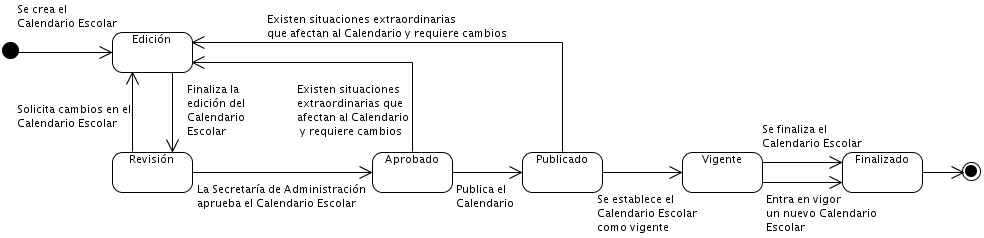
\includegraphics[width=\textwidth]{images/maquinasEstados/maquinaEstadosCalendario.png}}
			\caption{Modelo del ciclo de vida del calendario escolar - ciclo escolar.}
			\label{fig:maquinaEstadosCalendario}
		\end{figure}
		
		
		\BRterm{estado:edicion}{\bf Edición:} Es el estado inicial que se da cuando se crea el Calendario Escolar, en este estado la \cdtRef{Actor:CCE}{Coordinación de Control Escolar} puede realizar la gestión de las actividades del calendario escolar, agregando o eliminando actividades. Podrá cambiar al estado ''Revisión'' de acuerdo a la siguiente transición: 
		\begin{itemize}
			\item Finaliza la edición del Calendario Escolar. Una vez que la \cdtRef{Actor:CCE}{Coordinación de Control Escolar} ha terminado la edición de las actividades el Calendario cambiará al estado ''Revisión'' .
		\end{itemize}
		
		
		\BRterm{estado:revision}{\bf Revisión:} En este estado la \cdtRef{Actor:SA}{Secretaría de Administración} únicamente puede revisar el calendario generado por la \cdtRef{Actor:CCE}{Coordinación de Control Escolar}. Podrá cambiar al estado ''Edición'' o ''Aprobado'' de acuerdo a las siguientes transiciones: 
		\begin{itemize}
			\item Solicita cambios en el Calendario Escolar. Si la \cdtRef{Actor:SA}{Secretaría de Administración} ha encontrado inconsistencias o solicita que se realicen modificaciones, el Calendario cambiará al estado ''Edición''.
			\item La Secretaría de Administración aprueba el Calendario Escolar. Si la \cdtRef{Actor:SA}{Secretaría de Administración} considera que el calendario escolar no requiere cambios y lo aprueba, el Calendario cambiará al estado ''Aprobado''.
		\end{itemize}
		
		
		\BRterm{estado:aprobado}{\bf Aprobado:}  En este estado, el Calendario Escolar ha sido aprobado por la \cdtRef{Actor:SA}{Secretaría de Administración} y ya no se requieran modificaciones. Podrá cambiar al estado ''Edición'' o ''Publicado'' de acuerdo a las siguientes transiciones: 
		\begin{itemize}
			\item Existen situaciones extraordinarias que afectan a Calendario y requieren cambios. En caso de que se requieran realizar cambios en el Calendario por situaciones que se presenten después de haber sido aprobado, el Calendario cambiará al estado ''Edición''.
			\item Publica el Calendario. Una vez que la \cdtRef{Actor:CCE}{Coordinación de Control Escolar} decide publicar el Calendario, éste cambiará al estado ''Publicado''.
		\end{itemize}
		
		\BRterm{estado:publicado}{\bf Publicado:} En este estado el Calendario Escolar es puesto a disposición de la comunidad de la Escuela Libre de Derecho. Podrá cambiar al estado ''Edición'' o ''Vigente'' de acuerdo a las siguientes transiciones: 
		\begin{itemize}
			\item Existen situaciones extraordinarias que afectan a Calendario y requieren cambios. En caso de que se requieran realizar cambios en el Calendario por situaciones que se presenten después de haber sido publicado, el Calendario cambiará al estado ''Edición''.
			\item Se establece el Calendario Escolar como vigente. Cuando se desee establecer como vigente, cambiará al estado ''Vigente''.
		\end{itemize}
		
		\BRterm{estado:vigente}{\bf Vigente:} En este estado la \cdtRef{Actor:CCE}{Coordinación de Control Escolar} no puede registrar más grupos, únicamente puede editar la información, configurar horarios y visualizarlos. Únicamente la \cdtRef{Actor:SA}{Secretaría de Administración} puede realizar alguna modificación cuando el Calendario se encuentra en este estado. No puede haber más de un Calendario Escolar en este estado. Podrá cambiar al estado ''Finalizado'' de acuerdo a las siguientes transiciones: 
		\begin{itemize}
			\item Se finaliza el Calendario Escolar. Cuando la \cdtRef{Actor:CCE}{Coordinación de Control Escolar} considera que el Calendario terminó y desea finalizarlo, el Calendario cambiará al estado ''Finalizado''.
			\item Entra en vigor un nuevo Calendario Escolar. Cuando otro Calendario Escolar cambie de estado a ''Vigente'', el Calendario que se encontraba en este estado cambiará al estado ''Finalizado''.
		\end{itemize}
		
		\BRterm{estado:finalizado}{\bf Finalizado:} Es el estado final del Calendario, en este estado el Calendario Escolar queda finalizado quedando como registro histórico.
		
	}
	\BRitem{Referenciado por}{\cdtIdRef{CUPA1.1-1}{Gestionar ciclos escolares}}
	

\subsection{Habilitación de Acciones}
La tabla \ref{tb:iconosCicloEscolarA} \cdtRef{tb:iconosCicloEscolarA}{Acciones para Ciclos Escolares} muestra la forma en que se habilitarán las acciones en la gestión de ciclos escolares para la \cdtRef{Actor:CCE}{Coordinación de Control Escolar}. Las acciones se mostrarán con base en el estado que se encuentre cada ciclo escolar.\\

\begin{table} 
	\begin{center}
		\begin{tabular}{|l|l|l|l|l|l|l|l|}
			\hline
%			Estado/Operación  & \btnGestionar & \btnEditar &  \cdtButton{Registrar} & \btnBorrar &\btnVer &\btnCheck &\btnVigente \\
			\hline \hline
			Edición & Habilitado & Habilitado & Habilitado & Habilitado & Deshabilitado & Deshabilitado & Deshabilitado\\ \hline
			Revisión & Deshabilitado & Deshabilitado & Deshabilitado & Deshabilitado & Habilitado & Deshabilitado & Deshabilitado\\ \hline
			Aprobado & Deshabilitado & Deshabilitado & Deshabilitado & Deshabilitado & Habilitado & Habilitado & Deshabilitado\\ \hline
			Publicado & Deshabilitado & Deshabilitado & Deshabilitado & Deshabilitado & Habilitado & Habilitado & Habilitado\\ \hline
			Vigente & Deshabilitado & Deshabilitado & Deshabilitado & Deshabilitado & Deshabilitado & Habilitado & Deshabilitado\\ \hline
			Finalizado & Deshabilitado & Deshabilitado & Deshabilitado & Deshabilitado & Habilitado& Deshabilitado & Deshabilitado\\ \hline
		\end{tabular}
		\caption{Acciones para gestionar Ciclos Escolares para la Coordinación de Control Escolar.}
		\hypertarget{tb:habilitarAcciones}{}
		\label{tb:iconosCicloEscolarA}
	\end{center}
\end{table}


\subsection{Habilitación de Acciones}
La tabla \ref{tb:iconosCicloEscolarB} \cdtRef{tb:iconosCicloEscolarA}{Acciones para Ciclos Escolares} muestra la forma en que se habilitarán las acciones en la gestión de ciclos escolares para la \cdtRef{Actor:SA}{Secretaría de Administración}. Las acciones se mostrarán con base en el estado que se encuentre cada ciclo escolar.\\

\begin{table} 
	\begin{center}
		\begin{tabular}{|l|l|l|l|l|l|}
			\hline
%			Estado/Operación & \btnVer & \btnError & \btnRegresarConvocatoria & \btnEditar & \btnVigente \\
			\hline \hline
			Edición & Deshabilitado & Deshabilitado &  Deshabilitado &  Deshabilitado &  Deshabilitado\\ \hline
			Revisión & Habilitado & Deshabilitado & Habilitado &  Deshabilitado &  Deshabilitado\\ \hline
			Aprobado & Habilitado & Deshabilitado & Habilitado &  Deshabilitado &  Deshabilitado\\ \hline
			Publicado & Habilitado & Habilitado & Habilitado &  Deshabilitado &  Habilitado\\ \hline
			Vigente & Habilitado & Habilitado & Habilitado &  Habilitado &  Deshabilitado\\ \hline
			Finalizado & Habilitado & Deshabilitado & Deshabilitado &  Deshabilitado &  Deshabilitado\\ \hline
		\end{tabular}
		\caption{Acciones para gestionar Ciclos Escolares para la Secretaría de Administración.}
		\hypertarget{tb:habilitarAcciones}{}
		\label{tb:iconosCicloEscolarB}
	\end{center}
\end{table}	


\end{BusinessRule}

%criterios asociados a la convocatoria
\begin{BusinessRule}{RN-N3}{Criterios asociados a una convocatoria de ingreso}
	{Derivación}
	%se cambió el nombre de la regla de 
	{Controla la operación}
	\BRitem{Versión}{1.0}
	\BRitem{Autor}{Eduardo Espino Maldonado}
	\BRitem{Estatus}{Edición}
	\BRitem{Descripción}{

		Se define como criterio a todo aquello que se considera en la calificación para ingreso a la Escuela Libre de Derecho, por lo que requiere de una definición de valores (mínimo y máximo) así como la ponderación (en porcentaje) correspondiente en la convocatoria de ingreso. Dado que estos pueden variar entre convocatorias de ingreso, siempre se debe cumplir que:

		
		\begin{equation}
		    \sum_{i=1}^{i=n}C_i=100
		\end{equation}
		
		
		En donde: \\
		\begin{itemize}
		    \item $C_i$ es la ponderación asignada al criterio $i$
		    \item $n$ es la cantidad total de criterios asociados a la convocatoria de ingreso
		\end{itemize}
	}
	\BRitem{Referenciado por}{\cdtIdRef{CUPA1.2-2}{Gestionar criterios}}
\end{BusinessRule}

\begin{BusinessRule}{RN-N4}{Periodo válido}
%se cambió el nombre de la regla de negocio
	{Derivación}
	{Controla la operación}
	\BRitem{Versión}{1.0}
	\BRitem{Autor}{Eduardo Espino Maldonado}
	\BRitem{Estatus}{Edición}
	\item[Descripción:] 
	Para el registro de actividades en las cuales contengan actividades contenidas en un periodo, se debe cumplir lo siguiente.
	
	Un periodo definido tiene:\\
	\begin{center}
        $P_d = [f_{ini},f_{fin}] $ \\	
	\end{center}

	en donde:\\
	\begin{itemize}
	    \item $f_{ini}$: Fecha de inicio del periodo
	    \item $f_{fin}$: Fecha de término del periodo
	\end{itemize}
	
	y se debe cumplir lo siguiente:

	\begin{enumerate}
	    \item $f_{ini} < f_{fin}$ \\
	
		dadas las siguientes condiciones:
		\begin{itemize}
		    \item $f_{fin} \geq f_{ini}+60$
		    \item $f_{fin} \leq f_{ini}+365$
        \end{itemize}		
		\item  Al establecer la fecha de inicio del ciclo escolar:
		\begin{verbatim}fechaRegistroDeCiclo < fechaInicioDeCiclo\end{verbatim}
		\item  Al establecer la fecha de publicación:
		\begin{verbatim}fechaInicioDeCiclo >= fechaPublicacion\end{verbatim}
		
	\end{enumerate}
	%La duración mínima de un ciclo es de 60 días y máxima de 365 días

	\BRitem{Referenciado por}{\cdtIdRef{CUPA1.1-3}{Editar ciclo escolar}, \cdtIdRef{CUPA1.1-4}{Registrar ciclo escolar}, \cdtIdRef{CUGA7.4-3.1}{Registrar ausencia temporal}, \cdtIdRef{CUGA7.4-3.2}{Editar ausencia temporal}.}
\end{BusinessRule}

\begin{BusinessRule}{RN-N5}{Cálculo de la lista de calificaciones de los aspirantes}
	{Derivación}
	%Se cambió el nombre a la regla de negocio y se escribió mas detallada
	{Controla la operación}
	\BRitem{Versión}{1.0}
	\BRitem{Autor}{Eduardo Espino Maldonado}
	\BRitem{Estatus}{Edición}
	\item[Descripción:] 
	La calificación para el ingreso a la ELD de cada aspirante, se calcula de la siguiente manera:
	\[
	PG=\sum_{i=1}^n CalC_{i}\cdot {C_{i}}
	\]
	En donde: 
	\begin{itemize}
		\item $CalC_{i}$: Calificación obtenida por el aspirante para el criterio $i$
		\item $C_i$ = Ponderación del criterio $i$
		\item $n$: Número de criterios asociados a la convocatoria de ingreso
	\end{itemize}
	\BRitem{Referenciado por}{\cdtIdRef{CUPA1.8.1-1}{Generar lista de aspirantes para entrevistar}, \cdtIdRef{CUPA1.9-1}{Configurar lista de aspirantes}, \cdtIdRef{CUPA1.9-2}{Agregar aspirantes a la lista de aceptados},}
\end{BusinessRule}

%\begin{BusinessRule}{RN-N6}{Fechas de registro de actividades}
%	{Derivación}
%	{Controla la operación}
%	\BRitem{Versión}{1.0}
%	\BRitem{Autor}{Eduardo Espino Maldonado}
%	\BRitem{Estatus}{Edición}
%	\item[Descripción:] Solo pueden registrarse actividades de un ciclo escolar con base en la siguiente fórmula: 
%	\begin{verbatim}
%	fechaInicioDeCiclo <= fechaInicioDeActividad <= fechaTerminoDeActividad
%	<= fechaTerminoDeCiclo
%	\end{verbatim}
%	\item[Parámetros:]
%	\begin{itemize}
%		\item fechaInicioDeCiclo = Fecha de inicio del ciclo escolar.
%		\item fechaInicioDeActividad = Fecha de inicio de la actividad.
%		\item fechaTerminoDeActividad = Fecha de término de la actividad.
%		\item fechaTerminoDeCiclo = Fecha de término del ciclo escolar.
%	\end{itemize}
%	\BRitem{Referenciado por}{\cdtIdRef{CUPA1.1-5}{Editar actividad}, \cdtIdRef{CUPA1.1-6}{Registrar actividad},\cdtIdRef{CUPA1.2-8}{Registrar periodo},\cdtIdRef{CUPA1.2-9}{Editar periodo}, \cdtIdRef{CUPA1.1-14}{Editar actividad al ciclo escolar}}
%\end{BusinessRule}
%
%\begin{BusinessRule}{RN-N7}{Registro de horarios para actividades}
%	%se cambió el nombre de la regla de negocio y se generalizó
%	{Derivación}
%	{Controla la operación}
%	\BRitem{Versión}{1.0}
%	\BRitem{Autor}{Oscar Eduardo García García}
%	\BRitem{Estatus}{Edición}
%	\item[Descripción:] Una actividad está definida como una fecha o un periodo que puede tener un horario que comprende hora de inicio y hora de término. Sea un par de actividades  cualesquieran $C_A$ y $C_B$, en donde $C_A$ = $C_B$ que tienen un horario, se debe cumplir que:
%	
%	\begin{center}
%		$ \{ \{C_{Afin} \geq C_{Bini} \} \&\& \{C_{Aini} \leq C_{Bfin}\} 
%		\} \neq true$ 
%	\end{center}
%En donde:
%	\begin{itemize}
%		\item $C_{Aini}$: Hora de inicio de la actividad $A$
%		\item $C_{Afin}$: Hora de fin de la actividad $A$
%		\item $C_{Bini}$: Hora de inicio de la actividad $B$
%		\item $C_{Bfin}$: Hora de fin de la  actividad $B$	
%	\end{itemize}
%
%	El horario de una actividad es opcional, pero en caso de que se ingrese la hora de inicio, la hora de término será obligatoria y viceversa.
%	
%	\BRitem{Referenciado por}{\cdtIdRef{CUPA1.2-8}{Registrar periodo}, \cdtIdRef{CUPA1.2-9}{Editar periodo}, \cdtIdRef{CUPA1.8.4-1}{Seleccionar horario de entrevista}, \cdtIdRef{CUPA1.8.3-3}{Administrar horarios del entrevistador}}
%\end{BusinessRule}
%
%\begin{BusinessRule}{RN-N8}{Ciclo de vida de una convocatoria de ingreso}
%	{Derivación}
%	{Controla la operación}
%	\BRitem{Versión}{1.0}
%	\BRitem{Autor}{Brenda Gómez Caballero}
%	\BRitem{Estatus}{Edición}
%	\BRitem{Descripción}{
%	Una convocatoria de ingreso puede pasar por una serie de etapas o 'estados' en el sistema, los cuales se asignan desde que es creada por la \cdtRef{Actor:CCE}{Coordinación de Control Escolar} hasta su publicación. El ciclo de vida de una convocatoria, sus estados y transiciones se muestran en la figura \ref{fig:maquinaEstadosConvocatoria} y se describen a continuación.
%	\begin{figure}[htbp!]
%		\centering
%		\fbox{\includegraphics[width=\textwidth]{images/maquinasEstados/maquinaEstadosConvocatoria}}
%		\caption{Modelo del ciclo de vida de convocatoria de ingreso.}
%		\label{fig:maquinaEstadosConvocatoria}
%	\end{figure}
%
%
%	 \BRterm{estado:edicion}{\bf Edición:} Este es el estado inicial, y es en donde la  \cdtRef{Actor:CCE}{Coordinación de Control Escolar} puede realizar las configuraciones para la convocatoria de ingreso, agregando criterios, requisitos y actividades. Este estado es el inicio de las transiciones hacia los estados:
%	
%	\begin{itemize}
%		\item Revisión, una vez que la \cdtRef{Actor:CCE}{Coordinación de Control Escolar} ha terminado de configurar la convocatoria de ingreso. 
%	\end{itemize}
%	
%	
%	%estado de revisión
%	\BRterm{estado:revision}{\bf Revisión:} En este estado la \cdtRef{Actor:SA}{Secretaría de Administración} únicamente puede revisar la convocatoria de ingreso generada por la \cdtRef{Actor:CCE}{Coordinación de Control Escolar}. Este estado es el inicio de las transiciones hacia los estados:
%	\begin{itemize}
%		\item Edición, si la \cdtRef{Actor:SA}{Secretaría de Administración} ha encontrado inconsistencias o requiere modificaciones en la convocatoria de ingreso.
%		
%		\item Aprobada, si la convocatoria de ingreso no requiere cambios. 
%	\end{itemize}
%	
%	
%	\BRterm{estado:aprobada}{\bf Aprobada:} La convocatoria de ingreso pasa a este estado una vez que ya no se requieran modificaciones. Este estado es el inicio de las transiciones hacia los estados:
%	\begin{itemize}
%		\item Publicada, una vez que la fecha de publicación  establecida, en la convocatoria de ingreso, se alcanzó.
%		\item Edición, si se detectan inconsistencias en la convocatoria de ingreso y requiere cambios.
%	\end{itemize}
%	
%	\BRterm{estado:publicada}{\bf Publicada:} En este estado, la convocatoria es publicada. Este estado es el inicio de las transiciones hacia los estados:
%	\begin{itemize}
%		\item Edición, si durante la ejecución de las actividades de la convocatoria de ingreso se requiere realizar un cambio no previsto.
%		\item Cerrada, finaliza la convocatoria y la  \cdtRef{Actor:SA}{Secretaría de Administración} solicita cerrarla.
%	\end{itemize}
%
%	\BRterm{estado:cerrada}{\bf Cerrada:} La convocatoria de ingreso pasa a este estado una vez que la \cdtRef{Actor:SA}{Secretaría de Administración} la cierra manualmente. Este estado no genera transiciones a otros estados
%	}
%	\BRitem{Referenciado por}{\cdtIdRef{CUPA1.2-12}{Visualizar convocatoria de ingreso}, \cdtIdRef{CUPA1.2-13}{Aprobar convocatoria de ingreso}, \cdtIdRef{CUPA1.2-21}{Editar convocatoria de ingreso}}
%	
%	
%	\subsection{Habilitación de Acciones}
%	La tabla \ref{tb:iconosConvocatoriaA} \cdtRef{tb:iconosConvocatoriaA}{Acciones para convocatorias de ingreso}. muestra la forma en que se habilitarán las acciones en la gestión de convocatorias de ingreso para la \cdtRef{Actor:CCE}{Coordinación de Control Escolar}. Las acciones se mostrarán con base en el estado que se encuentre cada convocatoria de ingreso.\\
%	
%	\begin{table} 
%		\begin{center}
%			\begin{tabular}{|l|l|l|l|l|l|l|}
%				\hline
%				Estado/Operación & \cdtButton{Registrar} & \btnEditar & \btnGestionar & \btnVistaPrevia & \btnCheck & \btnBorrar \\
%				\hline \hline 
%				Edición & Habilitado & Habilitado & Habilitado  & Habilitado & Deshabilitado & Habilitado\\ \hline
%				Revisión & Habilitado & Deshabilitado & Deshabilitado  & Habilitado & Deshabilitado & Deshabilitado \\ \hline
%				Aprobada & Habilitado & Deshabilitado & Deshabilitado & Habilitado & Habilitado & Deshabilitado \\ \hline
%				Publicada & Habilitado & Habilitado & Deshabilitado & Habilitado & Deshabilitado & Deshabilitado \\ \hline
%				Cerrada & Habilitado & Habilitado & Deshabilitado & Habilitado & Deshabilitado & Deshabilitado \\ \hline
%			\end{tabular}
%			\caption{Acciones para gestionar Convocatorias de Ingreso para la Coordinación de Control Escolar.}
%			\hypertarget{tb:iconosConvocatoriaA}{}
%			\label{tb:iconosConvocatoriaA}
%		\end{center}
%	\end{table}	
%
%
%La tabla \ref{tb:iconosConvocatoriaB} \cdtRef{tb:iconosConvocatoriaB}{Acciones para convocatorias de ingreso}. muestra la forma en que se habilitarán las acciones en la gestión de convocatorias de ingreso para la \cdtRef{Actor:SA}{Secretaría de Administración}. Las acciones se mostrarán con base en el estado que se encuentre cada convocatoria de ingreso.\\
%
%\begin{table} 
%	\begin{center}
%		\begin{tabular}{|l|l|l|l|l|l|l|}
%			\hline
%			Estado/Operación & \btnVer & \btnVistaPrevia & \btnRegresarConvocatoria & \btnCerrarConvocatoria \\
%			\hline \hline 
%			Edición & Habilitado & Deshabilitado & Deshabilitado  & Deshabilitado \\ \hline
%			Revisión & Habilitado & Habilitado & Deshabilitado  & Deshabilitado   \\ \hline
%			Aprobada & Habilitado & Deshabilitado & Habilitado & Deshabilitado  \\ \hline
%			Publicada & Habilitado & Deshabilitado & Habilitado & Habilitado \\ \hline
%			Cerrada & Habilitado & Deshabilitado & Deshabilitado & Deshabilitado  \\ \hline
%		\end{tabular}
%		\caption{Acciones para gestionar Convocatorias de Ingreso para la Coordinación de Control Escolar.}
%		\hypertarget{tb:iconosConvocatoriaB}{}
%		\label{tb:iconosConvocatoriaB}
%	\end{center}
%\end{table}	
%
%\end{BusinessRule}
%
%\begin{BusinessRule}{RN-N9}{Medios de contacto registrados para un aspirante}
%	%Se cambió el nombre de la regla de negocio
%	{Derivación}
%	{Controla la operación}
%	\BRitem{Versión}{1.0}
%	\BRitem{Autor}{Adrian Flores Torres}
%	\BRitem{Estatus}{Edición}
%	\BRitem{Descripción}{Todo Aspirante a la ELD debe tener registrados mínimo:	\begin{itemize}
%		\item Un teléfono tipo personal.
%		\item Un teléfono tipo celular.
%		\item Un contacto de categoría emergencia.
%	\end{itemize}	
%	}
%	\BRitem{Referenciado por}{\cdtIdRef{CUPA1.4-5}{Registrar medios de contacto}}
%\end{BusinessRule}
%
%\begin{BusinessRule}{RN-N10}{Requisitos obligatorios de la convocatoria de ingreso}
%	{Derivación}
%	{Controla la operación}
%	\BRitem{Versión}{1.0}
%	\BRitem{Autor}{Brenda Gómez Caballero}
%	\BRitem{Estatus}{Edición}
%	\BRitem{Descripción}{Se consideran como requisitos obligatorios, para cualquier convocatoria de ingreso: 
%	\begin{itemize}
%	    \item Acta de nacimiento: La proporciona el aspirante, dado que es información personal.
%	    \item CURP: La proporciona el aspirante, dado que es información personal.
%	    
%	\end{itemize}
%	}
%	\BRitem{Referenciado por}{\cdtIdRef{CUPA1.2-13}{Aprobar convocatoria de ingreso}}
%\end{BusinessRule}
%
%\begin{BusinessRule}{RN-N11}{Periodo de Registro de Aspirantes}
%	{Derivación}
%	{Controla la operación}
%	\BRitem{Versión}{1.0}
%	\BRitem{Autor}{Brenda Gómez Caballero}
%	\BRitem{Estatus}{Edición}
%	\BRitem{Descripción}{El periodo para registro de aspirantes se define por la actividad marcada en el calendario escolar como Registro de Aspirantes especificada en la convocatoria.}
%	\BRitem{Referenciado por}{\cdtIdRef{CUPA1.3-2}{Crear cuenta},}
%\end{BusinessRule}
%
%
%\begin{BusinessRule}{RN-N12}{Ciclo de vida del aspirante}
%	{Derivación}
%	{Controla la operación}
%	\BRitem{Versión}{1.0}
%	\BRitem{Autor}{Brenda Gómez Caballero}		%%Carlos Alberto Granados Puerto
%	\BRitem{Estatus}{Edición}
%	\BRitem{Descripción}{
%	Un \cdtRef{Actor:Aspirante}{Aspirante} puede atravesar por diferentes ''estados'' a lo largo de su proceso de admisión a la ELD. Dependiendo del ''estado'' en que se encuentre podrá realizar diferentes actividades. Para cambiar de un estado a otro se debe realizar una transición, que se da cuando se cumple una condición.
%
%	Los estados y transiciones asociados al \cdtRef{Actor:Aspirante}{Aspirante} se describen a continuación junto a la Figura \ref{fig:maquinaEstadosAspirante}.
%	
%	\begin{figure}[htbp!]
%		\centering
%		\fbox{\includegraphics[width=\textwidth]{images/maquinasEstados/maquinaEstadosAspiranteV2}}
%		\caption{Ciclo de vida del aspirante.}
%		\label{fig:maquinaEstadosAspirante}
%	\end{figure}
%	
%	\BRterm{estado:preregistrado}{\bf Pre-registrado:} Es el estado inicial en el que se encuentra el \cdtRef{Actor:Aspirante}{Aspirante} una vez que crea su cuenta. Deberá ingresar al sistema mediante el link enviado a su correo para registrar su contraseña y activar su cuenta. Podrá avanzar a los estados que se mencionan a continuación conforme las siguientes transiciones:
%	
%	    \begin{itemize}
%			\item Error en el correo. En caso de que el aspirante ingresará erróneamente su correo electrónico y no se haya activado la cuenta, avanzará al mismo estado ''Pre-registrado''.
%		    \item Registra contraseña. Una vez que haya registrado la contraseña de su cuenta avanzará al estado ''Activado''.
%	    \end{itemize}
%
%	\BRterm{estado:activado}{\bf Activado:} En este estado se mostrará la pantalla \cdtIdRef{IU1.3-2A}{Bienvenido Aspirante}. Podrá avanzar al estado ''Condiciones aceptadas'' de acuerdo a la siguiente transición:
%	
%	    \begin{itemize}
%		    \item Acepta términos y condiciones. Una vez que haya aceptado los términos y condiciones bajo los cuales se llevará a cabo el proceso de admisión podrá avanzar al estado ''Condiciones aceptadas''.
%	    \end{itemize}
%
%	\BRterm{estado:condicionesAceptadas}{\bf Condiciones aceptadas:} En este estado se mostrará la pantalla \cdtIdRef{IU1.4}{Registro de Aspirantes}. Podrá avanzar al estado ''Registrado'' de acuerdo a la siguiente transición:
%
%	    \begin{itemize}
%		    \item Proporciona información. Una vez que el \cdtRef{Actor:Aspirante}{Aspirante} ha proporcionado la información requerida se concluye su registro pasando al estado ''Registrado''.
%	    \end{itemize}
%
%	\BRterm{estado:registrado}{\bf Registrado:} En este estado mostrará la pantalla \cdtIdRef{IU1.5-1A}{Pago de Derechos}. Podrá avanzar a los estados que se mencionan a continuación conforme las siguientes transiciones:
%	
%	    \begin{itemize}
%		    \item Acepta términos y condiciones de pagos. Una vez que el \cdtRef{Actor:Aspirante}{Aspirante} ha aceptado los términos y condiciones relacionados con los pagos avanzará al estado ''Pago de derechos''.
%		    \item No hay pago. En caso de que se determine que no se le cobrará al aspirante su derecho a evaluaciones avanzará directamente al estado ''Evaluaciones''.
%		    \item No hay evaluaciones ni pago. En caso de que se determine que no habrá evaluaciones para seleccionar al aspirante a entrevista y no se le cobrará cuota alguna para realizar la entrevista, avanzará directamente al estado ''Entrevista''.
%		    \item No hay evaluaciones, entrevistas ni pago. En caso de que se determine que sólo se seleccionará al aspirante conforme su promedio de secundario y bachillerato y no habrá cuota alguna para el proceso de admisión, avanzará directamente al estado ''Espera de resultados''.
%	    \end{itemize}
%
%	\BRterm{estado:pagoderechos}{\bf Pago de derechos:} En este estado el \cdtRef{Actor:aspirante}{Aspirante} deberá realizar el pago de derechos para tener derecho a presentar las evaluaciones. En este estado se mostrará la \cdtIdRef{IU1.5-1B}{Realizar Pago}. Podrá avanzar a los estados que se mencionan a continuación conforme las siguientes transiciones:
%	
%	    \begin{itemize}
%		    \item Realiza el pago de derechos. Una vez que el \cdtRef{Actor:Aspirante}{Aspirante} ha pagado podrá ser programado para presentar las evaluaciones y es notificado mediante un correo electrónico con el mensaje \cdtIdRef{MSG12}{Confirmación de pago}. Pasa al estado ''Evaluaciones''.
%		    \item No hay evaluaciones. Se dice que el \cdtRef{Actor:Aspirante}{Aspirante} ha pagado su derecho a realizar únicamente entrevista y es notificado mediante un correo electrónico con el mensaje \cdtIdRef{MSG12}{Confirmación de pago}. Pasa al estado ''Entrevista''.
%	    \end{itemize}
%	
%	\BRterm{estado:evaluaciones}{\bf Evaluaciones:} En este estado el \cdtRef{Actor:Aspirante}{Aspirante} presentará las evaluaciones correspondientes indicadas en la convocatoria. Se mostrará la pantalla \cdtIdRef{IU1.5-1C}{Evaluaciones}. Podrá avanzar a los estados que se mencionan a continuación conforme las siguientes transiciones:
%
%	    \begin{itemize}
%		    \item Se genera lista de aspirantes aceptados. Una vez que hayan terminado las evaluaciones se ordenan a los aspirantes de acuerdo al promedio alcanzado y se seleccionan N (configurado en la Convocatoria de ingreso) aspirantes con mejor promedio. El \cdtRef{Actor:Aspirante}{Aspirante} pasa al estado ''Entrevista''.
%		    \item No hay entrevistas. Una vez que hayan terminado las evaluaciones pasa directamente al estado ''Espera de resultados''.
%	    \end{itemize}
%
%
%	\BRterm{estado:entrevista}{\bf Entrevista:} En este estado el \cdtRef{Actor:Aspirante}{Aspirante} presenta la entrevista con el personal de la ELD. Se mostrará la pantalla \cdtIdRef{IU1.8.4-1}{Entrevista}. Podrá avanzar al estado ''Entrevista'' de acuerdo a la siguiente transición:
%
%	    \begin{itemize}
%		    \item Termina la entrevista. Una vez que se haya presentado la entrevista pasa al estado ''Espera de resultados''.
%	    \end{itemize}
%
%	\BRterm{estado:resultados}{\bf Espera de resultados:} En este estado se mostrará la pantalla \cdtIdRef{IU1.9-5}{Resultados}. El \cdtRef{Actor:Aspirante}{Aspirante} podrá avanzar al estado ''Aceptado'' de acuerdo a la siguiente transición:
%
%	\begin{itemize}
%		\item Recibe el resultado. Una vez que se haya aceptado al \cdtRef{Actor:Aspirante}{Aspirante} y notificado mediante un correo \cdtIdRef{MSG93}{Correo de aspirante aceptado}, pasa al estado ''Aceptado''.
%	\end{itemize}
%	
%	\BRterm{estado:aceptado}{\bf Aceptado:} En este estado el \cdtRef{Actor:Aspirante}{Aspirante} ha sido aceptado en la ELD por lo que podrá realizar su inscripción. Se mostrará la pantalla \cdtIdRef{IU1.9-6}{Aspirante Aceptado} en la que se mostrará su resultado obtenido al concluir el proceso de admisión.
%}
%	\BRitem{Referenciado por}{\cdtIdRef{CUPA1.3-2}{Crear cuenta}, \cdtIdRef{CUPA1.5-2}{Realizar pago con tarjeta}, \cdtIdRef{CUPA1.5-3}{Realizar pago OXXO/SPEI}, \cdtIdRef{CUPA1.3-1}{Iniciar Sesión}.}
%\end{BusinessRule}
%
%
%\begin{BusinessRule}{RN-N13}{Criterios obligatorios de la convocatoria de ingreso}
%	{Habilitador}
%	{Controla la operación}
%	\BRitem{Versión}{1.0}
%	\BRitem{Autor}{Diego Efrén Pascual Hernández}
%	\BRitem{Estatus}{Edición}
%	\BRitem{Descripción}
%	{Para toda convocatoria se consideran criterios obligatorios a:
%	\begin{itemize}
%	    \item Promedio general de secundaria
%	    \item Promedio general de bachillerato o equivalente
%	\end{itemize}
%	Para el caso de los aspirantes con estudios en el extranjero, se considerará 8.0 como valor para ambos criterios.
%}
%	\BRitem{Referenciado por}{}
%\end{BusinessRule}
%
%\begin{BusinessRule}{RN-N14}{Promedio general de ingreso de un aspirante}
%	{Derivación}
%	{Controla la operación}
%	\BRitem{Versión}{1.0}
%	\BRitem{Autor}{Eduardo Espino Maldonado}
%	\BRitem{Estatus}{Edición}
%	\item[Descripción:] El promedio mínimo para ingresar a la ELD se define por:\\
%	\begin{center}
%	$P_{Gral} = \frac{P_{S}+P_{B}}{2}$	
%	\end{center}
%
%
%	En donde: 
%	\begin{itemize}
%	    \item $P_{S}$: Promedio general de la secundaria
%    	\item $P_{B}$: Promedio general del bachillerato o equivalente 
%	\end{itemize}
%	
%	Y se debe cumplir que: 
%	\begin{center}
%	    	$P_{Gral} \geq P_{Min}$\\
%	\end{center}
%
%En donde el $P_{Min}$ se define en la convocatoria.
%
%
%
%	\BRitem{Referenciado por}{\cdtIdRef{CUPA1.4-7}{Registrar información escolar},}
%\end{BusinessRule}
%
%\begin{BusinessRule}{RN-N15}{Tiempo de entrevista}
%	{Derivación}
%	{Controla la operación}
%	\BRitem{Versión}{1.0}
%	\BRitem{Autor}{Oscar Eduardo García García}
%	\BRitem{Estatus}{Edición}
%	\BRitem{Descripción}{El tiempo de cada entrevista está definido por periodos de 20 minutos}
%	\BRitem{Referenciado por}{\cdtIdRef{CUPA1.8.4-1}{Seleccionar horario de entrevista}}
%\end{BusinessRule}
%
%\begin{BusinessRule}{RN-N16}{Unicidad de Elementos}
%	{Derivación}
%	{Controla la operación}
%	\BRitem{Versión}{1.0}
%	\BRitem{Autor}{Carlos Robles Ruiz}
%	\BRitem{Estatus}{Edición}
%	\BRitem{Descripción}{Un elemento no se puede duplicar en todo el sistema, ni registrar más de una ocasión. La unicidad se determinará con base en la siguiente lista:
%		\\ 
%			\begin{enumerate}
%			\item Aspirante:
%				\begin{itemize}
%					\item CURP
%				\end{itemize}
%			\item Etapa de un tipo de actividades
%				\begin{itemize}
%					\item Nombre, en el ámbito del tipo de actividades al que pertenece
%				\end{itemize}	
%			\item Actividad de una etapa:
%				\begin{itemize}
%					\item Nombre, en el ámbito de la etapa a la que pertenece
%				\end{itemize}
%			\item Criterio:
%				\begin{itemize}
%					\item Nombre
%				\end{itemize}
%			\item Requisito:
%				\begin{itemize}
%					\item Nombre
%				\end{itemize}
%			\item Convocatoria:
%				\begin{itemize}
%					\item Nombre
%				\end{itemize}
%		
%			%\item Para la entidad \textbf{Piscólogo:}
%			%\\
%			%\begin{UClist}
%			%	\UCli Registro de un Psicólogo. 
%			%\end{UClist}
%		
%			\item Plan de Estudios:
%			\begin{itemize}
%				\item Nombre
%				\item Fecha de entrada en vigor
%			\end{itemize}
%		
%			\item Materia:
%			\begin{itemize}
%				\item Nombre
%			\end{itemize}
%		
%			\item Grupo:
%			\begin{itemize}
%				\item Nombre
%			\end{itemize}
%		
%			\item Salón:
%			\begin{itemize}
%				\item Nombre
%			\end{itemize}
%		
%			\item Profesor:
%			\begin{itemize}
%				\item CURP
%				\item Correo electrónico
%				\item Usuario HandPunch
%			\end{itemize}
%		
%			\item Psicólogo:
%			\begin{itemize}
%				\item CURP
%			\end{itemize}
%		
%			\item Vigencia:
%			\begin{itemize}
%				\item Fecha de inicio
%				\item Fecha de término
%			\end{itemize}
%		
%			\item Concepto:
%			\begin{itemize}
%				\item Nombre
%			\end{itemize}
%			
%			\item Correo electrónico:
%			\begin{itemize}
%				\item Dirección de correo electrónico
%			\end{itemize}
%		\end{enumerate}
%	
%	Las actividades antes mencionadas, son las principales que utilizan esta regla de negocio. 
%	}
%
%	\BRitem{Referenciado por}{\cdtIdRef{CUPA1.2-3}{Agregar Criterio}, \cdtIdRef{CUPA1.2-5}{Agregar requisito}, \cdtIdRef{CUPA1.2-6}{Editar requisito}, \cdtIdRef{CUPA1.2-8}{Agregar periodo}, \cdtIdRef{CUPA1.2-9}{Editar periodo}, \cdtIdRef{CUPA1.2-15}{Configurar Criterio}, \cdtIdRef{CUPA1.2-20}{Registrar convocatoria de ingreso}, \cdtIdRef{CUPA1.2-21}{Editar convocatoria de ingreso}, \cdtIdRef{CUEA2.3}{Registrar Plan de estudios}, \cdtIdRef{CUEA2.4}{Editar plan de estudios}, \cdtIdRef{CUEA2.16}{Editar materia}}, \cdtIdRef{CUEA2.8}{Registrar Configuración de Equivalencias}, \cdtIdRef{CUEA2.13}{Registrar Materias Hijo}, \cdtIdRef{CUGA7.1-2}{Registrar grupo}, \cdtIdRef{CUGA7.1-3}{Editar grupo}, \cdtIdRef{CUGA7.2-2}{Registrar salón}, \cdtIdRef{CUGA7.2-3}{Editar salón}, \cdtIdRef{CUGA7.3-2}{Registrar profesor}, \cdtIdRef{CUGA7.3-2-1}{Crear cuenta}, \cdtIdRef{CUGA7.3-3}{Editar profesor}.
%\end{BusinessRule}
%
%\begin{BusinessRule}{RN-N17}{Criterios de origen para la convocatoria de ingreso}
%	{Derivación}
%	{Controla la operación}
%	\BRitem{Versión}{1.0}
%	\BRitem{Autor}{Fabiola Jaramillo Loredo}
%	\BRitem{Estatus}{Edición}
%	\BRitem{Descripción}{Una convocatoria de ingreso debe contener al menos las siguientes actividades registradas: 
%	\begin{itemize}
%		\item Registro de aspirantes
%		\item Periodo de Pago de exámenes
%		\item Periodo de aplicación del EXANI-II asociado al criterio CENEVAL
%		\item Aplicación de examen psicométrico asociado al criterio psicométrico
%		\item Aplicación de entrevistas asociado al criterio entrevistas
%		\item Publicación de resultados
%	\end{itemize}
%	Por lo que estas actividades no podrán ser eliminadas del catálogo.
%	}
%	\BRitem{Referenciado por}{\cdtIdRef{CUPA1.1-11}{Gestionar etapas}}
%\end{BusinessRule}
%
%
%
%%\begin{BusinessRule}{RN-N1}{Consultar calendarios}
%%	{Derivación}
%%	{Controla la operación}
%%	\BRitem{Versión}{1.0}
%%	\BRitem{Autor}{Eduardo Espino Maldonado}
%%	\BRitem{Estatus}{Terminado}
%%	\BRitem{Descripción}{Se mostrarán solamente los últimos 3 ciclos que ya han sido concluidos}
%%	\BRitem{Referenciado por}{{CUPA1.1-1}{Gestionar ciclos}
%%	}
%%\end{BusinessRule}
%
%%\begin{BusinessRule}{RN-N6}{Fecha de registro de un ciclo escolar}
%%	{Derivación}
%%	{Controla la operación}
%%	\BRitem{Versión}{1.0}
%%	\BRitem{Autor}{Eduardo Espino Maldonado}
%%	\BRitem{Estatus}{Edición}
%%	\item[Descripción:] La fecha de registro de un ciclo escolar debe cumplir con la siguiente fórmula:
%%		\begin{verbatim}
%%		fechaInicioDeCiclo > fechaRegistroDeCiclo
%%		\end{verbatim}
%%	\item[Descripción:]
%%		\begin{itemize}
%%			\item fechaInicioDeCiclo = Fecha de inicio del ciclo.
%%			\item fechaRegistroDeCiclo = Fecha en la cual se está registrando el ciclo
%%		\end{itemize}
%%	\BRitem{Referenciado por}{\cdtIdRef{CUPA1.1-3}{Editar ciclo escolar}, \cdtIdRef{CUPA1.1-4}{Registrar ciclo escolar},}
%%\end{BusinessRule}
%
%%\begin{BusinessRule}{RN-N5}{Operaciones permitidas de un ciclo escolar}
%%	{Derivación}
%%	{Controla la operación}
%%	\BRitem{Versión}{1.0}
%%	\BRitem{Autor}{Eduardo Espino Maldonado}
%%	\BRitem{Estatus}{Edición}
%%	\BRitem{Descripción}{No se podrá editar y/o eliminar un ciclo escolar que haya concluido, así como tampoco gestionar sus actividades}
%%	\BRitem{Referenciado por}{}
%%\end{BusinessRule}
%
%%\begin{BusinessRule}{RN-N8}{Duración de ciclo}
%%	{Derivación}
%%	{Controla la operación}
%%	\BRitem{Versión}{1.0}
%%	\BRitem{Autor}{Eduardo Espino Maldonado}
%%	\BRitem{Estatus}{Edición}
%%	\BRitem{Descripción}{La duración mínima de un ciclo es de 2 meses y máxima de 365 días}
%%	\BRitem{Referenciado por}{\cdtIdRef{CUPA1.1-3}{Editar ciclo}, \cdtIdRef{CUPA1.1-4}{Registrar ciclo},}
%%\end{BusinessRule}
%
%%\begin{BusinessRule}{RN-N11}{Valor mínimo del criterio}
%%	{Derivación}
%%	{Controla la operación}
%%	\BRitem{Versión}{1.0}
%%	\BRitem{Autor}{Oscar Eduardo García García}
%%	\BRitem{Estatus}{Edición}
%%	\item[Descripción:] El valor mínimo ingresado siempre debe de ser menor al valor máximo, con base en la siguiente fórmula: 
%%	\begin{verbatim}
%%	valorMinimo <= valorMaximo
%%	\end{verbatim}
%%	\item[Parámetros:]
%%	\begin{itemize}
%%		\item valorMinimo = Valor mínimo.
%%		\item valorMaximo = Valor máximo.
%%	\end{itemize}
%%	\BRitem{Referenciado por}{\cdtIdRef{CUPA1.2-11}{Asignar Configuración General}, \cdtIdRef{CUPA1.2-15}{Configurar Criterio}}
%%\end{BusinessRule}
%
%%\begin{BusinessRule}{RN-N20}{Alumno con baja definitiva o académica}
%%	{Derivación}
%%	{Controla la operación}
%%	\BRitem{Versión}{1.0}
%%	\BRitem{Autor}{Brenda Gómez Caballero}
%%	\BRitem{Estatus}{Edición}
%%	\BRitem{Descripción}{El alumno que se encuentra en el estado de una Baja Definitiva o Baja Académica, no puede volver a participar en ningún proceso de la Escuela Libre de Derecho}∫
%%	\BRitem{Referenciado por}{\cdtIdRef{CUPA1.3-2}{Crear cuenta}}
%%\end{BusinessRule}
%
%%% Esta no es una regla de negocio, es una definición del Actor: Aspirante
%%\begin{BusinessRule}{RN-N21}{Perfil del aspirante}
%%	{Derivación}
%%	{Controla la operación}
%%	\BRitem{Versión}{1.0}
%%	\BRitem{Autor}{Brenda Gómez Caballero}
%%	\BRitem{Estatus}{Edición}
%%	\BRitem{Descripción}{Se considera aspirante a la persona que quiere ingresar a la Escuela Libre de Derecho, que no es estudiante de licenciatura y no ha causado baja definitiva dentro de la institución}
%%	\BRitem{Referenciado por}{\cdtIdRef{CUPA1.3-2}{Crear cuenta},}
%%\end{BusinessRule}
%
%%\begin{BusinessRule}{RN-N35}{Número de alumnos por salón para examen CENEVAL}
%%	{Derivación}
%%	{Controla la operación}
%%	\BRitem{Versión}{1.0}
%%	\BRitem{Autor}{Carlos Alberto Robles Ruiz}
%%	\BRitem{Estatus}{Edición}
%%	\item[Descripción:]{Los salones dedicados para aplicar el examen CENEVAL tienen una capacidad descrita en la siguiente ecuación}:
%%	
%%	\begin{itemize}	
%%		\item Se definen los siguientes parámetros:
%%		\begin{itemize}
%%			\item \textbf{Ct} es la capacidad total que un salón posee.
%%			\item \textbf{Ca} es la cantidad de aspirantes del salón para el examen CENEVAL.
%%		\end{itemize}
%%		\item La capacidad de alumnos es estrictamente menor que la capacidad total del salón: 
%%		\begin{equation}
%%		1 < Ca < Ct   
%%		\end{equation}
%%	\end{itemize}	
%%	\BRitem{Referenciado por}{}
%%\end{BusinessRule}
%%
%%
%%\begin{BusinessRule}{RN-N36}{Salones suficientes para examen CENEVAL}
%%	{Derivación}
%%	{Controla la operación}
%%	\BRitem{Versión}{1.0}
%%	\BRitem{Autor}{Carlos Alberto Robles Ruiz}
%%	\BRitem{Estatus}{Edición}
%%	\item[Descripción:] {El total de la capacidad de los salones seleccionados para aplicar el examen CENEVAL deben cubrir al menos la cantidad de folios solicitados, tal como se describe en la siguiente ecuación}:
%%	\begin{itemize}	
%%		\item Se definen los siguientes parámetros:
%%		\begin{itemize}
%%			\item \textbf{Ss} es la cantidad de salones seleccionados.
%%			\item \textbf{Ce} es la capacidad del examen CENEVAL del salón. 
%%			\item \textbf{Fs} es el total de folios solicitados al CENEVAL.
%%		\end{itemize}
%%		\item Se debe cumplir que: 
%%		\begin{equation}
%%		Ss * Ce => Fs
%%		\end{equation}
%%	\end{itemize}	
%%	\BRitem{Referenciado por}{}
%%\end{BusinessRule}
%%
%%
%%\begin{BusinessRule}{RN-N}{Encuesta CENEVAL obligatoria}
%%	{Derivación}
%%	{Controla la operación}
%%	\BRitem{Versión}{1.0}
%%	\BRitem{Autor}{Carlos Alberto Robles Ruiz}
%%	\BRitem{Estatus}{Edición}
%%	\BRitem{Descripción}{Para obtener un registro ante CENEVAL, los aspirantes deben de responder la encuesta CENEVAL que se les proporciona}
%%	\BRitem{Referenciado por}{}
%%\end{BusinessRule}
%
%%\begin{BusinessRule}{RN-N43}{Cantidad de aspirantes agregados permitidos}
%%	{Derivación}
%%	{Controla la operación}
%%	\BRitem{Versión}{1.0}
%%	\BRitem{Autor}{Diego Efrén Pascual Hernández}
%%	\BRitem{Estatus}{Edición}
%%	\BRitem{Descripción}{La cantidad máxima de aspirantes que se pueden agregar de la lista de aceptados son 260 aspirantes.}
%%	\BRitem{Referenciado por}{}
%%\end{BusinessRule}
%%
%%\begin{BusinessRule}{RN-N44}{Cantidad de aspirantes eliminados permitidos}
%%	{Derivación}
%%	{Controla la operación}
%%	\BRitem{Versión}{1.0}
%%	\BRitem{Autor}{Diego Efrén Pascual Hernández}
%%	\BRitem{Estatus}{Edición}
%%	\BRitem{Descripción}{La cantidad mínima de aspirantes que se pueden agregar de la lista de aceptados son 240 aspirantes.}
%%	\BRitem{Referenciado por}{}
%%\end{BusinessRule}
%
%%\begin{BusinessRule}{RN-N45}{Lista de Aceptados}
%%	{Derivación}
%%	{Controla la operación}
%%	\BRitem{Versión}{1.0}
%%	\BRitem{Autor}{}
%%	\BRitem{Estatus}{Edición}
%%	\BRitem{Descripción}{Lista de aspirantes aceptados se ordena de forma ascendente con base en el promedio general}
%%	\BRitem{Referenciado por}{}
%%\end{BusinessRule}
%
%
%%\begin{BusinessRule}{RN-N46}{Lista de no Aceptados}
%%	{Derivación}
%%	{Controla la operación}
%%	\BRitem{Versión}{1.0}
%%	\BRitem{Autor}{}
%%	\BRitem{Estatus}{Edición}
%%	\BRitem{Descripción}{Lista de aspirantes no aceptados se ordena de forma descendente con base en el promedio general}
%%	\BRitem{Referenciado por}{}
%%\end{BusinessRule}
%
%%\begin{BusinessRule}{RN-N47}{Lista de Ciclos}
%%	{Derivación}
%%	{Controla la operación}
%%	\BRitem{Versión}{1.0}
%%	\BRitem{Autor}{Adrian Flores Torres}
%%	\BRitem{Estatus}{Edición}
%%	\BRitem{Descripción}{Lista de los ciclos se ordena de forma descendente con base en la fecha mas reciente}
%%	\BRitem{Referenciado por}{}
%%\end{BusinessRule}
%
%%\begin{BusinessRule}{RN-N49}{Cantidad de alumnos aceptados}
%%	{Derivación}
%%	{Controla la operación}
%%	\BRitem{Versión}{1.0}
%%	\BRitem{Autor}{Brenda Gómez Caballero}
%%	\BRitem{Estatus}{Edición}
%%	\BRitem{Descripción}{La cantidad máxima de alumnos aceptados debe ser CMÁXIMA.}
%%	\item[Parámetros:] El mensaje se muestra con base en los siguientes parámetros:
%%	\begin{Citemize} 
%%		\item CMÁXIMA: Se establece en la convocatoria.
%%	\end{Citemize}
%%	\BRitem{Referenciado por}{\cdtIdRef{CUPA1.2-11}{Asignar configuración general}, \cdtIdRef{CUPA1.9-2}{Agregar aspirantes a la lista de aceptados}, }
%%\end{BusinessRule}
%
%\begin{BusinessRule}{RN-N18}{Ciclo de vida de la cuenta del Profesor}
%	{Derivación}
%	{Controla la operación}
%	\BRitem{Versión}{1.0}
%	\BRitem{Autor}{Liliana Flores Sánchez}
%	\BRitem{Estatus}{Edición}
%	\BRitem{Descripción}{
%		Una cuenta puede pasar por una serie de etapas o 'estados' en el sistema. Dependiendo del estado, el actor puede realizar diferentes actividades. Los estados y transiciones se muestran en la figura \ref{fig:maquinaEstadosCuentaProfesor} y se describen a continuación.
%		
%		\begin{figure}[htbp!]
%			\centering
%			\fbox{\includegraphics[scale=.5]{images/maquinasEstados/maquinaEstadosCuentaProfesor}}
%			\caption{Modelo del ciclo de vida de la cuenta del Profesor.}
%			\label{fig:maquinaEstadosCuentaProfesor}
%		\end{figure}
%
%	\BRterm{estado:activo}{\bf Activo:}  El \cdtRef{Actor:profesor}{Profesor} toma este estado cuando es registrado. Un profesor en este estado puede ser seleccionado para horarios, exámenes profesionales. Este estado es el inicio de las transiciones hacia los estados: 
%	\begin{itemize}
%		\item \textbf{Inactivo parcial.} Pasa a este estado cuando se registra una licencia o ausencia.
%		\item \textbf{Inactivo total.} Pasa a este estado cuando el \cdtRef{Actor:profesor}{Profesor} pide una renuncia definitiva, es destituido o fallece.
%	\end{itemize}
%
%	\BRterm{estado:inactivoParcial}{\bf Inactivo parcial:} El \cdtRef{Actor:profesor}{Profesor} se encuentra en este estado durante el tiempo en que su licencia o ausencia está vigente. En este estado el profesor no puede participar en ningún proceso de  la ELD. Este estado es el inicio de las transiciones hacia los estados: 
%	\begin{itemize}
%		\item \textbf{Activo.} Pasa a este estado una vez que el tiempo de licencia o ausencia se ha cumplido.
%		\item \textbf{Inactivo total.} Pasa a este estado cuando el \cdtRef{Actor:profesor}{Profesor} pide una renuncia definitiva, es destituido o fallece.
%	\end{itemize}
%	
%	
%	\BRterm{estado:inactivoTotal}{\bf Inactivo total:} El profesor se encuentra en este estado a partir de la fecha de registro del evento de fallecimiento, destitución o renuncia definitiva. Los profesores en este estado no pueden participar en ningún proceso de la ELD. Este es un estado terminal.
%}	
%	\BRitem{Referenciado por}{\cdtIdRef{CUGA7.3-2-1}{Crear cuenta}.}
%\end{BusinessRule}
%
%\begin{BusinessRule}{RN-N19}{Ciclo de vida de la cuenta del Alumno}
%	{Derivación}
%	{Controla la operación}
%	\BRitem{Versión}{1.0}
%	\BRitem{Autor}{Liliana Flores Sánchez}
%	\BRitem{Estatus}{Edición}
%	\BRitem{Descripción}{
%		Una cuenta puede pasar por una serie de etapas o 'estados' en el sistema. Dependiendo del estado, el actor puede realizar diferentes actividades. Los estados y transiciones se muestran en la figura \ref{fig:maquinaEstadosCuentaAlumno} y se describen a continuación.
%		
%		\begin{figure}[htbp!]
%			\centering
%			\fbox{\includegraphics[scale=.5]{images/maquinasEstados/maquinaEstadosCuentaAlumno}}
%			\caption{Modelo del ciclo de vida de la cuenta del Alumno.}
%			\label{fig:maquinaEstadosCuentaAlumno}
%		\end{figure}
%		
%		\BRterm{estado:alumnoActivo}{\bf Activo:} El \cdtRef{Actor:alumno}{Alumno} En este estado se encuentran todos los alumnos inscritos en la ELD, a cualquier grado de su programa de Derecho. 
%		\begin{itemize}
%			\item \textbf{Baja temporal.} Pasa a este estado cuando la ELD aprueba la solicitud de baja temporal.
%			\item \textbf{Baja definitiva.} Pasa a este estado cuando fallece.
%			\item \textbf{Baja académica.} Pasa a este estado cuando cumple con alguno de los siguientes puntos:
%			\begin{itemize}
%				\item Repruebe tres veces la misma materia. 
%				\item No acredite tres exámenes correspondientes al primer curso. Se entenderá por no acreditar tanto reprobar como no presentar el examen final correspondiente por causa injustificada a juicio de la Junta Directiva.
%				\item Repruebe cuatro veces en las mismas o distintas materias durante los primeros dos cursos.
%				\item Repruebe cinco veces en las mismas o distintas materias en el curso de los años primero a tercero.
%				\item Repruebe seis veces en las mismas o distintas materias a lo largo de su carrera.				
%			\end{itemize}
%			\item \textbf{Egresado.} Pasa a este estado cuando ha aprobado todas sus materias.
%		\end{itemize}
%		
%		\BRterm{estado:bajaTemporal}{\bf Baja Temporal:} El \cdtRef{Actor:alumno}{Alumno} toma este estado cuando la ELD ha aprobado la solicitud de baja temporal, indicando un periodo definido, como se muestra en la siguiente fórmula:
%	
%%	FÓRMULA
%			Un periodo definido tiene:\\
%		\begin{center}
%			$P_d = [f_{ini},f_{fin}] $ \\	
%		\end{center}
%		
%		en donde:\\
%		\begin{itemize}
%			\item $f_{ini}$: Fecha de inicio del periodo
%			\item $f_{fin}$: Fecha de término del periodo
%		\end{itemize}
%		
%		El cambio de estado se realiza cuando:
%		\begin{center}
%			$f_{act} = f_{fin}$
%		\end{center}
%			
%		en donde: \\
%		\begin{itemize}
%			\item $f_{act}$: Fecha actual
%		\end{itemize}
%		
%		Este estado es el inicio de las transiciones hacia los estados:
%		\begin{itemize}
%			\item \textbf{Activo.} Pasa a este estado una vez que el periodo de baja temporal ha concluido.
%			\item \textbf{Baja definitiva.} Pasa a este estado cuando fallece.
%		\end{itemize}
%		
%		\BRterm{estado:bajaDefinitiva}{\bf Baja definitiva:} El \cdtRef{Actor:alumno}{Alumno} toma este estado cuando fallece. Este es un estado terminal.
%		
%		\BRterm{estado:bajaAcademica}{\bf Baja académica:} El \cdtRef{Actor:alumno}{Alumno} toma este estado cuando cumple con alguno de los siguientes puntos:
%		\begin{itemize}
%			\item Repruebe tres veces la misma materia. 
%			\item No acredite tres exámenes correspondientes al primer curso. Se entenderá por no acreditar tanto reprobar como no presentar el examen final correspondiente por causa injustificada a juicio de la Junta Directiva.
%			\item Repruebe cuatro veces en las mismas o distintas materias durante los primeros dos cursos.
%			\item Repruebe cinco veces en las mismas o distintas materias en el curso de los años primero a tercero.
%			\item Repruebe seis veces en las mismas o distintas materias a lo largo de su carrera.				
%		\end{itemize}
%		Este es un estado terminal.
%		
%		\BRterm{estado:egresado}{\bf Egresado:} El \cdtRef{Actor:alumno}{Alumno} toma este estado cuando ha aprobado todas las materias de la Licenciatura. 
%		
%		\BRterm{estado:titulado}{\bf Titulado:} El \cdtRef{Actor:alumno}{Alumno} toma este estado cuando ha aprobado el examen de titulación. Este es un estado terminal.
%	}	
%	\BRitem{Referenciado por}{}
%\end{BusinessRule}
%
%\begin{BusinessRule}{RN-N20}{Título de tratamiento de un profesor}
%	{Derivación}
%	{Controla la operación}
%	\BRitem{Versión}{1.0}
%	\BRitem{Autor}{Liliana Flores Sánchez}
%	\BRitem{Estatus}{Edición}
%	\BRitem{Descripción} {El título de tratamiento debe ser calculado con base en el género, el estado civil y el grado académico del profesor de la siguiente forma:
%		
%			\begin{center}
%				Titulo = [Título][EstadoCivil][TítuloNobiliario]
%			\end{center}
%			
%		En donde:
%		\begin{itemize}
%			\item Título: 
%				\begin{itemize}
%					\item Don: Para profesores del género masculino.
%					\item Doña: Para profesores del género femenino.
%				\end{itemize}
%			\item EstadoCivil:
%				\begin{itemize}
%					\item Sr.: Para profesores del género masculino, sin importar que sean solteros o casados.
%					\item Sra.: Para profesores del género femenino y casadas.
%					\item Srita.: Para profesores del género femenino y solteras.
%				\end{itemize}
%			\item TítuloNobiliario: Se tomará el grado de mayor jerarquía registrado en la Trayectoria Académica del profesor. Al registrar un profesor se tomará como grado académico el de Lic.
%				\begin{enumerate}
%					\item Dr.
%					\item Mtro.
%					\item Lic.
%				\end{enumerate}	
%		\end{itemize}
%}
%	\BRitem{Ejemplo}{
%		Para género masculino: Don Sr. Lic. Francisco López Huerta. Para género femenino soltera: Doña Srita. Mtra. Rosa Olivares Torres.
%	}
%			
%	\BRitem{Referenciado por}{}
%\end{BusinessRule}
%
%\begin{BusinessRule}{RN-N21}{Prioridad de domicilio para los profesores}
%	{Derivación}
%	{Controla la operación}
%	\BRitem{Versión}{1.0}
%	\BRitem{Autor}{Liliana Flores Sánchez}
%	\BRitem{Estatus}{Edición}
%	\BRitem{Descripción} {
%		
%		Los profesores deberán tener registrado un único domicilio marcado como prioritario.
%		}
%	\BRitem{Referenciado por}{\cdtIdRef{CUGA7.3-18}{Definir prioridad de domicilio}.}
%\end{BusinessRule}
%
%\begin{BusinessRule}{RN-N22}{Traslape de horario de materia}
%	{Derivación}
%	{Controla la operación}
%	\BRitem{Versión}{1.0}
%	\BRitem{Autor}{Liliana Flores Sánchez}
%	\BRitem{Estatus}{Edición}
%	
%	\item[Descripción:] {Se define como traslape de horario a: 
%		
%	Sean dos materias A y B, existe un traslape bajo las siguientes circunstancias:
%	
%	\begin{itemize}
%		
%	\item Traslape entre materias obligatorias iguales impartidas por el mismo profesor:
%		\begin{itemize}
%			\item Si A y B son obligatorias,			
%			\item A y B son iguales,
%			\item A y B son impartidas en diferentes grupos,
%			\item A y B son impartidas en el mismo horario y
%			\item A y B son impartidas por el mismo profesor.
%		\end{itemize}
%	\item Traslape entre materias obligatorias diferentes impartidas por el mismo profesor:
%		\begin{itemize}
%			\item Si A y B son obligatorias,			
%			\item A y B son diferentes,
%			\item A y B son impartidas en diferentes grupos o en el mismo grupo,
%			\item A y B son impartidas en el mismo horario y
%			\item A y B son impartidas por el mismo profesor.
%			
%		\end{itemize}
%	\item Traslape entre materias obligatorias diferentes impartidas por profesores diferentes:
%		\begin{itemize}
%			\item Si A y B son obligatorias,
%			\item A y B son diferentes,
%			\item A y B son impartidas en el mismo grupo, 
%			\item A y B son impartidas en el mismo horario y
%			\item A y B son impartidas por profesores diferentes.		
%		\end{itemize}
%
%	\item Traslape entre materias obligatoria y optativa, impartidas por el mismo profesor o diferentes
%	\begin{itemize}
%		\item Si A es una materia obligatoria y B es una materia optativa,		
%		\item A y B son impartidas en el mismo grupo y 
%		\item A y B son impartidas en el mismo horario 		
%	\end{itemize}
%	\end{itemize}
%		
%		
%	}
%	\BRitem{Referenciado por}{\cdtIdRef{CUGA7.1.1-2}{Agregar horario de grupo}, \cdtIdRef{CUGA7.1.1-4}{Editar horario de grupo}.}
%\end{BusinessRule}
%
%
%%PENDIENTE
%\begin{BusinessRule}{RN-N23}{Horas de una materia padre con hijos}
%	{Derivación}
%	{Controla la operación}
%	\BRitem{Versión}{1.0}
%	\BRitem{Autor}{Carlos Aníbal Larios Moguel}
%	\BRitem{Estatus}{Edición}
%	\BRitem{Descripción} {
%		
%		Sea A una materia padre que tiene por lo menos dos hijos, el número de horas de la materia A se definirá como:
%
%	\begin{equation}
%		    \sum_{i=1}^{i=n}Hh_i=Hp
%		\end{equation}
%		
%		
%		En donde: \\
%		\begin{itemize}
%		    \item $Hh_i$ es el número de horas(semana) de una materia hijo $i$
%		    \item $n$ es la cantidad total de materias hijo asociadas a la materia padre
%		    \item $Hp$ es la cantidad total de horas(semana) de la materia padre
%		\end{itemize}
%}
%	\BRitem{Referenciado por}{\cdtIdRef{CUEA2.16}{Editar materia}.}
%\end{BusinessRule}
%
%\begin{BusinessRule}{RN-N24}{Horas impartidas de clase por materia}
%	{Derivación}
%	{Controla la operación}
%	\BRitem{Versión}{1.0}
%	\BRitem{Autor}{Cesar Raúl Avila Padilla}
%	\BRitem{Estatus}{Edición}
%	\BRitem{Descripción} {Para calendarizar el horario de una materia M en un ciclo escolar, se debe cumplir que:
%		
%	\begin{center}	
%		$HM_s = HM = \sum_{i=1}^{i=n}H_{mi}$
%	\end{center}
%
%	En donde: \\
%	\begin{itemize}
%		\item $HM_s$ es la cantidad de horas programadas en el horario de la materia M para la semana.
%		\item $HM$ es la cantidad de horas de la materia, por semana, definidas en el plan de estudios.
%		\item $n$ es el número total de horarios definidos para la materia M.
%		\item $H_{mi}$ es la cantidad de horas definidas para el horario $i$
%\end{itemize}
%}
%	\BRitem{Referenciado por}{\cdtIdRef{CUGA7.1.1-2}{Agregar horario de grupo}, \cdtIdRef{CUGA7.1.1-4}{Editar horario de grupo}.}
%\end{BusinessRule}
%
%%PENDIENTE
%\begin{BusinessRule}{RN-N25}{Horario de clases para el ciclo escolar}
%	{Derivación}
%	{Controla la operación}
%	\BRitem{Versión}{1.0}
%	\BRitem{Autor}{Cesar Raúl Avila Padilla}
%	\BRitem{Estatus}{Edición}
%	\BRitem{Descripción} {El horario de una materia debe estar contenido en los periodos que comprenden los horarios (matutino y vespertino) definidos por la ELD.
%
%}
%	\BRitem{Referenciado por}{\cdtIdRef{CUGA7.1.1-2}{Agregar horario de grupo}, \cdtIdRef{CUGA7.1.1-4}{Editar horario de grupo}.}
%\end{BusinessRule}
%
%\begin{BusinessRule}{RN-N26}{Fecha para la entrada en vigor de un plan de estudios}
%	{Derivación}
%	{Controla la operación}
%	\BRitem{Versión}{1.0}
%	\BRitem{Autor}{Liliana Flores Sánchez}
%	\BRitem{Estatus}{Edición}
%	\BRitem{Descripción} {La fecha en la que un plan de estudios entra en vigor debe ser posterior a su fecha de registro.}
%	\BRitem{Referenciado por}{}
%\end{BusinessRule}
%
%\begin{BusinessRule}{RN-N27}{Restricciones para registrar materias hijo a materia padre}
%	{Derivación}
%	{Controla la operación}
%	\BRitem{Versión}{1.0}
%	\BRitem{Autor}{Carlos Aníbal Larios Moguel}
%	\BRitem{Estatus}{Edición}
%	\BRitem{Descripción} {Sea una materia M a la cual se le agregarán materias hijo: 
%		\begin{enumerate}
%			\item El número de materias hijo debe ser mayor a 1
%			\item Las materias hijo solo pueden ser registradas para una materia padre obligatoria.
%		\end{enumerate}
%		}
%	\BRitem{Referenciado por}{ \cdtIdRef{CUEA2.12}{Registrar materia}, \cdtIdRef{CUEA2.16}{Editar materia}}
%\end{BusinessRule}
%
%
%
%
%%\begin{BusinessRule}{RN-N28}{Equivalencias entre planes de estudio}
%%	{Derivación}
%%	{Controla la operación}
%%	\BRitem{Versión}{1.0}
%%	\BRitem{Autor}{Carlos Aníbal Larios Moguel}
%%	\BRitem{Estatus}{Edición}
%%	\BRitem{Descripción} {Dados dos planes de estudios registrados, plan A y plan B, las equivalencias entre los mismos se registrarán de la siguiente manera, de acuerdo a la máquina de estados:
%%		\begin{itemize}
%%			\item Para el plan A en estado 'Aprobado', sólo se podrán registrar equivalencias con el plan B 
%%			\begin{itemize}
%%				\item En estado 'Vigente'
%%				\item En estado 'de salida'
%%				\item En estado 'Histórico'
%%			\end{itemize} 
%%			\item Para el plan A en estado 'Vigente', sólo se podrán registrar equivalencias con el plan B 
%%			\begin{itemize}
%%				\item En estado 'de salida'
%%				\item En estado 'Histórico'
%%			\end{itemize}
%%			\item Para el plan A en estado 'de salida', sólo se podrán registrar equivalencias con el plan B 
%%			\begin{itemize}
%%				\item En estado 'Histórico'
%%			\end{itemize}
%%
%%		\end{itemize}
%%	}
%%	\BRitem{Referenciado por}{ \cdtIdRef{IUEA2.6}{Registrar equivalencia}}
%%\end{BusinessRule}
%
%\begin{BusinessRule}{RN-N28}{Equivalencias entre planes de estudio}
%	{Derivación}
%	{Controla la operación}
%	\BRitem{Versión}{1.0}
%	\BRitem{Autor}{Carlos Aníbal Larios Moguel}
%	\BRitem{Estatus}{Edición}
%	\BRitem{Descripción} {Dados dos planes de estudios registrados, plan A y plan B, las equivalencias entre los mismos se registrarán de la siguiente manera, de acuerdo a la máquina de estados:
%		\begin{itemize}
%			
%			\item Para el plan A en estado 'Vigente', sólo se podrán registrar equivalencias con el plan B 
%			\begin{itemize}
%				\item En estado 'Liquidación'
%				\item En estado 'Derogado'
%			\end{itemize}
%
%		\end{itemize}
%	}
%	\BRitem{Referenciado por}{ \cdtIdRef{IUEA2.6}{Registrar equivalencia}}
%\end{BusinessRule}
%
%\begin{BusinessRule}{RN-N29}{Ciclo de vida de un plan de estudios}
%	{Derivación}
%	{Controla la operación}
%	\BRitem{Versión}{0.1}
%	\BRitem{Autor}{Carlos Aníbal Larios Moguel}
%	\BRitem{Estatus}{Edición}
%	\BRitem{Descripción}{
%	Un plan de estudios puede pasar por una serie de etapas o 'estados' en el sistema, los cuales se asignan desde que es creado por la \cdtRef{Actor:CCE}{Coordinación de Control Escolar} hasta que pasa a ser parte del registro histórico. El ciclo de vida de un plan de estudios, sus estados y transiciones se muestran en la figura \ref{fig:maquinaEstadosPlanEstudios} y se describen a continuación.
%	\begin{figure}[htbp!]
%		\centering
%		\fbox{\includegraphics[width=\textwidth]{images/maquinasEstados/maquinaEstadosPlanesEstudios}}
%		\caption{Modelo del ciclo de vida de Planes de Estudios.}
%		\label{fig:maquinaEstadosPlanEstudios}
%	\end{figure}
%
%
%	 \BRterm{estado:edicion}{\bf Edición:} Este es el estado inicial, y es en donde la  \cdtRef{Actor:CCE}{Coordinación de Control Escolar} puede realizar la gestión del plan de estudio, este es el estado que toma un plan de estudios al ser registrado. Este estado es el inicio de las transiciones hacia los estados:
%	
%	\begin{itemize}
%		\item Revisión, una vez que la \cdtRef{Actor:CCE}{Coordinación de Control Escolar} ha terminado la gestión del plan de estudios. 
%	\end{itemize}
%	
%	
%	%estado de revisión
%	\BRterm{estado:revision}{\bf Revisión:} En este estado la \cdtRef{Actor:SA}{Secretaría de Administración} únicamente puede revisar el plan de estudios generado por la \cdtRef{Actor:CCE}{Coordinación de Control Escolar} para su aprobación o solicitud de cambios. Este estado es el inicio de las transiciones hacia los estados:
%	\begin{itemize}
%		\item Edición, si la \cdtRef{Actor:SA}{Secretaría de Administración} ha encontrado inconsistencias o se requieren modificaciones al plan de estudios.
%		
%		\item Aprobado, si el plan de estudios no requiere cambios. 
%	\end{itemize}
%	
%	
%	\BRterm{estado:aprobado}{\bf Aprobado:} El plan de estudios pasa a este estado una vez que ya no se requieren modificaciones. Este estado es el inicio de las transiciones hacia los estados:
%	\begin{itemize}
%		\item Vigente, una vez que la \cdtRef{Actor:SA}{Secretaría de Administración} determina que la fecha de entrada en vigor ha sido alcanzada.
%	\end{itemize}
%	
%	\BRterm{estado:vigente}{\bf Vigente:} En este estado la \cdtRef{Actor:SA}{Secretaría de Administración} o  la \cdtRef{Actor:CCE}{Coordinación de Control Escolar}   establece el plan de estudios como vigente, lo que implica que los alumnos podrán inscribir las materias correspondientes a dicho plan. No puede haber más de un plan de estudios en este estado. Este estado es el inicio de las transiciones hacia los estados:
%	\begin{itemize}
%		\item Liquidación, si un nuevo plan de estudios pasa al estado vigente.
%	\end{itemize}
%	
%	\BRterm{estado:liquidacion}{\bf Liquidación:} Una vez que un plan de estudios alcanza este estado, permanece ahí por un tiempo de n+1 ciclos escolares, siendo n el número de grados del plan de estudios. Además, los grupos que se inscribirán cada ciclo escolar cumplen con las siguientes condiciones:
%	\begin{itemize}
%		\item En el ciclo escolar que el plan de estudios entra en liquidación se inscriben los grupos que corresponden a los n grados.
%		\item A partir del segundo ciclo escolar hasta el ciclo escolar n se inscriben G grupos y en cada uno deja de inscribir el grupo del grado más bajo.
%		\[
%		G=\sum_{i=1}^m n-i
%		\]
%		Donde m es n-1.
%		\item En el ciclo escolar n+1, se inscribe nuevamente el grupo que corresponde al grado n.
%	\end{itemize}
%	Este estado es el inicio de las transiciones hacia los estados:
%	\begin{itemize}
%		\item Histórico, Cuando se cumplieron los n+1 ciclos escolares del plan de estudios en estado Liquidación.
%	\end{itemize}
%	
%	\BRterm{estado:historico}{\bf Derogado:} En este estado el plan de estudios únicamente puede ser consultado. Este es el estado final para un plan de estudios.
%	
%	}
%	\BRitem{Referenciado por}{\cdtIdRef{CUEA2.20}{Eliminar Plan de estudios}, \cdtIdRef{CUEA2.4}{Editar plan de estudios}, \cdtIdRef{CUEA2.18}{Aprobar Plan de Estudios}, \cdtIdRef{CUEA2.20}{Eliminar Plan de Estudios}, \cdtIdRef{CUGA7.1-2}{Registrar grupo}, \cdtIdRef{CUGA7.1-3}{Editar grupo}.}
%	
%	\subsection{Habilitación de Acciones}
%	La tabla \ref{tb:iconosPlanesEstudioCCE} \cdtRef{tb:iconosPlanesEstudioCCE}{Acciones para Planes de Estudios} muestra la forma en que se habilitarán las acciones en la gestión de planes de estudio para la \cdtRef{Actor:CCE}{Coordinación de Control Escolar}. Las acciones se mostrarán con base en el estado que se encuentre cada plan de estudios.\\
%	
%	\begin{table} 
%		\begin{center}
%			\begin{tabular}{|l|l|l|l|l|l|}
%				\hline
%				Estado/Operación  & \cdtButton{Registrar} & \btnEditar & \btnGestionar &  \btnVer & \btnBorrar \\
%				\hline \hline
%				Edición & Habilitado & Habilitado & Habilitado & Habilitado & Habilitado\\ \hline
%				Revisión & Deshabilitado & Deshabilitado & Deshabilitado & Habilitado & Deshabilitado\\ \hline
%				Aprobado & Deshabilitado & Deshabilitado & Deshabilitado & Habilitado & Deshabilitado\\ \hline
%				Vigente & Deshabilitado & Deshabilitado & Deshabilitado & Habilitado & Deshabilitado\\ \hline
%				Liquidación & Deshabilitado & Deshabilitado & Deshabilitado & Habilitado & Deshabilitado\\ \hline
%				Histórico & Deshabilitado & Deshabilitado & Deshabilitado & Habilitado & Deshabilitado\\ \hline
%			\end{tabular}
%			\caption{Acciones para gestionar Planes de Estudios para la Coordinación de Control Escolar.}
%			\hypertarget{tb:iconosPlanesEstudioCCE}{}
%			\label{tb:iconosPlanesEstudioCCE}
%		\end{center}
%	\end{table}
%	
%	
%	\subsection{Habilitación de Acciones}
%	La tabla \ref{tb:iconosPlanesEstudioSA} \cdtRef{tb:iconosPlanesEstudioSA}{Acciones para Planes de Estudios} muestra la forma en que se habilitarán las acciones en la gestión de planes de estudio para la \cdtRef{Actor:SA}{Secretaría de Administración}. Las acciones se mostrarán con base en el estado que se encuentre cada plan de estudios.\\
%	
%	\begin{table} 
%		\begin{center}
%			\begin{tabular}{|l|l|l|l|}
%				\hline
%				Estado/Operación & \btnEvaluacion & \btnVigente & \btnVer \\ \hline \hline
%				Edición & Deshabilitado & Deshabilitado & Habilitado\\ \hline
%				Revisión & Habilitado & Deshabilitado & Habilitado\\ \hline
%				Aprobado & Deshabilitado & Habilitado & Habilitado\\ \hline
%				Vigente & Deshabilitado & Deshabilitado & Habilitado\\ \hline
%				Liquidación & Deshabilitado & Deshabilitado & Habilitado\\ \hline
%				Histórico & Deshabilitado & Deshabilitado & Habilitado\\ \hline
%			\end{tabular}
%			\caption{Acciones para gestionar Planes de Estudios para la Secretaría de Administración.}
%			\hypertarget{tb:iconosPlanesEstudioSA}{}
%			\label{tb:iconosPlanesEstudioSA}
%		\end{center}
%	\end{table}
%
%\end{BusinessRule}
%
%\begin{BusinessRule}{RN-N30}{Cálculos para la generación de citas de examen psicométrico}
%	{Derivación}
%	{Controla la operación}
%	\BRitem{Versión}{1.0}
%	\BRitem{Autor}{Diego Efrén Pascual Hernández}
%	\BRitem{Estatus}{Edición}
%	\BRitem{Descripción}{Los recursos para generar citas para las actividades del examen psicométrico están definidos por lo siguiente:
%		\begin{itemize}
%			\item $JL = H_{fj} - H_{ij}$
%			\item $S = P + 4$
%			\item $C = 2 * P$
%			\item $BD = \frac{JL - D}{I}$
%			\item $BP = BD * DP$
%			\item $AB = 2 * C$
%			\item $AD = AB * BD$
%			\item $TE = \frac{I}{4}$
%			\item $TEE = \frac{I}{2}$
%			\item $THTP = \frac{I}{4}$
%			\item $AP = (JL - D) * DP$
%			\item $APE = AD * DP$
%		\end{itemize}
%	
%		En donde:
%		\begin{itemize}
%			\item $JL$ son las horas de la jornada laboral.
%			\item $H_{ij}$ es la hora de inicio de la jornada.
%			\item $H_{fj}$ es la hora de término de la jornada.
%			\item $S$ es el número de salones.
%			\item $P$ es el número de psicólogos.
%			\item $C$ es el número de computadoras.
%			\item $D$ es el número de horas de descanso.
%			\item $I$ es el número de horas de cada intervalo.
%			\item $BD$ es el número de bloques por día.
%			\item $DP$ es el número de días del periodo.
%			\item $BP$ es el número de bloques por periodo.
%			\item $AB$ es el número de aspirantes por bloque.
%			\item $AD$ es el número de aspirantes por día.
%			\item $TE$ es el tiempo que dura la entrevista.
%			\item $TEE$ es el tiempo que dura el examen electrónico.
%			\item $THTP$ es el tiempo que dura la prueba HTP.
%			\item $AP$ es el número de aspirantes que se le deben asignar a un psicólogo.
%			\item $APE$ es el número de aspirantes por periodo.
%		\end{itemize}
%	
%	}
%	\BRitem{Referenciado por}{}
%\end{BusinessRule}
%
%\begin{BusinessRule}{RN-N31}{Ciclo de vida de una equivalencia}
%	{Derivación}
%	{Controla la operación}
%	\BRitem{Versión}{1.0}
%	\BRitem{Autor}{María Elsi Bernabé Aparicio}
%	\BRitem{Estatus}{Edición}
%	\BRitem{Descripción}{Una equivalencia puede pasar por una serie de ''estados'' en el sistema. Dependiendo del estado, el actor puede realizar diferentes actividades. Los estados y transiciones se muestran en la figura \ref{fig:maquinaEstadosEquivalencia} y se describen a continuación.
%		\begin{figure}[htbp!]
%			\centering
%			\fbox{\includegraphics[width=\textwidth]{images/maquinasEstados/maquinaEstadosEquivalencia}}
%			\caption{Modelo del ciclo de vida de una equivalencia.}
%			\label{fig:maquinaEstadosEquivalencia}
%		\end{figure}
%		
%		%estado Edición
%		\BRterm{estado:edicion}{\bf Edición:} Pasa a este estado cuando la \cdtRef{Actor:CCE}{Coordinación de Control Escolar} registra las equivalencias de una materia con una o más de otro plan de estudios. Este estado es el inicio de las transiciones hacia los estados:
%
%		\begin{itemize}
%			\item Revisión, una vez que la \cdtRef{Actor:CCE}{Coordinación de Control Escolar} ha terminado de gestionar las equivalencias.
%		\end{itemize}
%				
%		%estado Revisión
%		\BRterm{estado:revision}{\bf Revisión:} En este estado la \cdtRef{Actor:SA}{Secretaría de Administración} revisa las equivalencias registradas por la \cdtRef{Actor:CCE}{Coordinación de Control Escolar}. Este estado es el inicio de las transiciones hacia los estados:
%		\begin{itemize}
%			\item Edición, si la \cdtRef{Actor:SA}{Secretaría de Administración} ha encontrado inconsistencias o requiere modificaciones.
%			
%			\item Aprobada, si la equivalencia no requiere cambios. 
%		\end{itemize}
%		
%		%estado Aprobada
%		\BRterm{estado:aprobado}{\bf Aprobado:} Pasa a este estado cuando la equivalencia se realizó correctamente y no requiere modificaciones. Este es el estado final para una equivalencia.
%	}
%	\BRitem{Referenciado por}{\cdtIdRef{CUEA2.7}{Gestionar equivalencias de materias},
%		\cdtIdRef{CUEA2.8}{Registrar equivalencia de materias}.}
%\end{BusinessRule}
%
%%\begin{BusinessRule}{RN-N31}{Conceptos críticos para psicométrico}
%%	{Derivación}
%%	{Controla la operación}
%%	\BRitem{Versión}{1.0}
%%	\BRitem{Autor}{Diego Efrén Pascual Hernández}
%%	\BRitem{Estatus}{Edición}
%%	\BRitem{Descripción}{Si se selecciona uno de los siguientes conceptos críticos, el resultado final cambiará a 'No aceptado':
%%		\begin{itemize}
%%			\item CONCEPTO A
%%			\item CONCEPTO B
%%			\item CONCEPTO C
%%		\end{itemize}
%%	}
%%	\BRitem{Referenciado por}{}
%%\end{BusinessRule}
%
%\begin{BusinessRule}{RN-N32}{Ponderación de evaluación psicométrica}
%	{Derivación}
%	{Controla la operación}
%	\BRitem{Versión}{1.0}
%	\BRitem{Autor}{Diego Efrén Pascual Hernández}
%	\BRitem{Estatus}{Edición}
%	\BRitem{Descripción}{El promedio final de la evaluación psicométrica esta dado por los siguientes casos:
%		\begin{itemize}
%			\item Aceptado = 10
%			\item Aceptado con reservas = 5
%			\item No aceptado = 0
%		\end{itemize}
%	}
%	\BRitem{Referenciado por}{}
%\end{BusinessRule}
%%
%%\begin{BusinessRule}{RN-N33}{Tarjetas válidas}
%%	{Derivación}
%%	{Controla la operación}
%%	\BRitem{Versión}{1.0}
%%	\BRitem{Autor}{Brenda Gómez Caballero}
%%	\BRitem{Estatus}{Edición}
%%	\BRitem{Descripción}{Las tarjetas que corresponde a la red global de MasterCard o Visa, son las únicas válidas para hacer los pagos.}
%%	\BRitem{Referenciado por}{\cdtIdRef{CUPA1.5-2}{Realizar pago con tarjeta} }
%%\end{BusinessRule}
%
%\begin{BusinessRule}{RN-N33}{Porcentaje del criterio de selección}
%	{Derivación}
%	{Controla la operación}
%	\BRitem{Versión}{1.0}
%	\BRitem{Autor}{Carlos Alberto Granados Puerto}
%	\BRitem{Estatus}{Edición}
%	\BRitem{Descripción}{
%		El porcentaje aportado por la calificación obtenida en el criterio se calcula de la siguiente manera:
%
%		\begin{equation}
%		    \% = P(R-R_{min})/(R_{max}-R_{min})
%		\end{equation}
%
%		Debe cumplir que: 
%		
%		\begin{equation}
%		    R_{min}<=R<=R_{max}
%		\end{equation}
%
%		En donde: \\
%		\begin{itemize}
%		  \item $R_{min}$ es el puntaje mínimo requerido
%		  \item $R_{max}$ es el puntaje máximo solicitado
%		  \item $P$ es la ponderación asignada al criterio
%		  \item $R$ es el resultado obtenido por el aspirante
%		\end{itemize}
%	}
%	\BRitem{Referenciado por}{\cdtIdRef{CUPA1.2-2}{Gestionar criterios}, \cdtIdRef{CUPA1.2-28}{Gestionar evaluaciones}.}
%\end{BusinessRule}
%
%\begin{BusinessRule}{RN-N34}{Tarjeta vigente}
%	{Derivación}
%	{Controla la operación}
%	\BRitem{Versión}{1.0}
%	\BRitem{Autor}{Brenda Gómez Caballero}
%	\BRitem{Estatus}{Edición}
%	\BRitem{Descripción}{Solo será válida la tarjeta que cumpla con la fechas permitidas con base en la siguiente fórmula: 
%		\begin{itemize}
%			\item $FVT > FA$
%		\end{itemize}
%		En donde: 
%		\begin{itemize}
%			\item $FVT$ es la fecha de vencimiento de la tarjeta con el formato MM/AA localizado en el anverso de la tarjeta.
%			\item $FA$ es la fecha en la que se está haciendo el registro para el pago correspondiente, tomando en cuenta desde 01/MM/AA.
%		\end{itemize}
%	}	
%	\BRitem{Referenciado por}{\cdtIdRef{CUPA1.5-2}{Realizar pago con tarjeta}}
%\end{BusinessRule}
%
%\begin{BusinessRule}{RN-N35}{Tiempo de vida de una referencia para pagos}
%	{Derivación}
%	{Controla la operación}
%	\BRitem{Versión}{1.0}
%	\BRitem{Autor}{Brenda Gómez Caballero}
%	\BRitem{Estatus}{Edición}
%	\BRitem{Descripción}{La caducidad de la referencia para los pagos en SPEI y OXXO se calculará con base en la siguiente fórmula: 					
%		\begin{itemize}
%			\item $FC < FTPP - 1$
%		\end{itemize}
%		En donde:
%		\begin{itemize}
%			\item $FC$ es la fecha de vencimiento de la referencia para los pagos en SPEI y OXXO.
%			\item $FTPP$ es la fecha en la que concluye el período permitido para el pago correspondiente.
%		\end{itemize}
%	}
%	\BRitem{Referenciado por}{\cdtIdRef{CUPA1.5-3}{Realizar pago OXXO/SPEI}}
%\end{BusinessRule}
%
%\begin{BusinessRule}{RN-N36}{Eliminar medios de contacto}
%	{Derivación}
%	{Controla la operación}
%	\BRitem{Versión}{1.0}
%	\BRitem{Autor}{Brenda Gómez Caballero}
%	\BRitem{Estatus}{Edición}
%	\BRitem{Descripción}{Sólo puede eliminarse un medio de contacto si existe al menos uno en cada uno de los siguientes tipos: 'Personal' y 'Trabajo'.}
%	\BRitem{Referenciado por}{\cdtIdRef{CUGA7.3-15}{Eliminar medio de contacto} }
%\end{BusinessRule}
%
%%\begin{BusinessRule}{RN-N38}{Materias Padre}
%%	{Derivación}
%%	{Controla la operación}
%%	\BRitem{Versión}{1.0}
%%	\BRitem{Autor}{Larios Moguel Carlos Aníbal}
%%	\BRitem{Estatus}{Edición}
%%	\BRitem{Descripción}{Sólo las materias obligatorias pueden tener materias hijo.}
%%	\BRitem{Referenciado por}{\cdtIdRef{CUEA2.12}{Registrar materia}, \cdtIdRef{CUEA2.16}{Editar materia} }
%%\end{BusinessRule}
%
%\begin{BusinessRule}{RN-N37}{Registro de nuevo plan de estudios}
%	{Derivación}
%	{Controla la operación}
%	\BRitem{Versión}{1.0}
%	\BRitem{Autor}{Larios Moguel Carlos Aníbal}
%	\BRitem{Estatus}{Edición}
%
%	\BRitem{Descripción}{Al registrar un plan de estudios nuevo, se debe realizar una copia de la siguiente información del plan de estudios actualmente vigente:
%
%		\begin{itemize}
%			\item Niveles del plan de estudios
%			\item Materias por nivel del plan de estudios
%			\item Atributos de las materias del plan de estudios
%		\end{itemize}}
%	\BRitem{Referenciado por}{\cdtIdRef{CUEA2.3}{Registrar plan de estudios} }
%\end{BusinessRule}
%
%\begin{BusinessRule}{RN-N38}{Nombre de plan de estudios}
%	{Derivación}
%	{Controla la operación}
%	\BRitem{Versión}{1.0}
%	\BRitem{Autor}{Larios Moguel Carlos Aníbal}
%	\BRitem{Estatus}{Edición}
%	\BRitem{Descripción}{Al registrar un nuevo plan de estudios, el nombre se calculará de la siguiente manera: 
%			$Nombre=Plan+AAAA$
%			En donde:
%			\begin{itemize}
%				\item $AAAA$: Es el año de la fecha de entrada en vigor registrado para el plan de estudios. 
%			\end{itemize}
%			
%		}
%	\BRitem{Referenciado por}{\cdtIdRef{CUEA2.3}{Registrar plan de estudios}}
%\end{BusinessRule}
%
%\begin{BusinessRule}{RN-N39}{Medios de contacto registrados para un profesor}
%	{Derivación}
%	{Controla la operación}
%	\BRitem{Versión}{1.0}
%	\BRitem{Autor}{Adrian Flores Torres}
%	\BRitem{Estatus}{Edición}
%	\BRitem{Descripción}{Todo profesor de la ELD debe tener registrados mínimo:	\begin{itemize}
%			\item Un teléfono tipo personal.
%			\item Un teléfono tipo trabajo.
%		\end{itemize}	
%	}
%	\BRitem{Referenciado por}{\cdtIdRef{CUGA7.3-8}{Gestionar medios de contacto}}
%\end{BusinessRule}
%
%
%\begin{BusinessRule}{RN-N40}{Traslape de periodos}
%	{Habilitadora}
%	{Controla la operación}
%	\BRitem{Versión}{1.0}
%	\BRitem{Autor}{Eduardo Espino Maldonado}
%	\BRitem{Estatus}{Edición}
%	\BRitem{Descripción}{Al registrar una ausencia temporal esta debe cumplir con lo siguiente:	
%		
%		Sea un par de periodos de ausencias temporales cualesquiera, $A_A$ y $A_B$, en donde $A_A \neq A_B$ se debe cumplir que: 
%
%		$$ \{ \{A_{Afin} \geq A_{Bini} \} \&\& \{A_{Aini} \leq A_{Bfin}\} \} \neq true$$
%		
%		en donde:
%		
%		\begin{itemize}
%			\item $A_{Aini}$: Fecha de inicio del periodo $A$ y debe ser mayor a la  actual.
%			\item $A_{Afin}$: Fecha de fin del periodo $A$
%			\item $A_{Bini}$: Fecha de inicio del periodo $B$ y debe ser mayor a la fecha actual.
%			\item $A_{Bfin}$: Fecha de fin del periodo $B$
%		\end{itemize}
%	}
%	\BRitem{Referenciado por}{\cdtIdRef{CUGA7.4-3.1}{Registrar ausencia temporal}, \cdtIdRef{CUGA7.4-3.2}{Editar ausencia temporal}.}
%\end{BusinessRule}
%
%
%\begin{BusinessRule}{RN-N41}{Fechas establecidas para convocatoria}
%	{Derivación}
%	{Controla la operación}
%	\BRitem{Versión}{1.0}
%	\BRitem{Autor}{Diana Guadalupe Maldonado Ledo}
%	\BRitem{Estatus}{Edición}
%	\BRitem{Descripción} La fecha de inicio y la fecha de término de una actividad de la convocatoria de ingreso, debe estar dentro del ciclo escolar, este se determina por:\\
%	\begin{center}
%		$\{ Act_{Convocatoria} - 2 sem \} < Fecha_{Ciclo Escolar}$	
%		\end{center}
%		
%		
%		En donde: 
%		\begin{itemize}
%		\item $A_{Convocatoria}$: Actividad de la Convocatoria de Ingreso
%		\item $Fecha_{ciclo escolar}$: Fecha de un ciclo escolar, por defecto desde el 31 de julio 
%		\end{itemize}
%		
%		Y se debe cumplir que la fecha de inicio y de término de la actividad de una Convocatoria de Ingreso debe ser menor a la fecha de inicio del ciclo escolar. En el caso de que no se tenga un periodo definido, se validará la fecha ingresada.
%		
%		\BRitem{Referenciado por}{}
%		\end{BusinessRule}
%
%
%
%\begin{BusinessRule}{RN-N42}{Traslape de ausencias de profesores con horarios de clases}
%	{Derivación}
%	{Controla la operación}
%	\BRitem{Versión}{1.0}
%	\BRitem{Autor}{Diana Guadalupe Maldonado Ledo}
%	\BRitem{Estatus}{Edición}
%	\BRitem{Descripción}{
%		Al registrar una ausencia temporal para un profesor, se debe verificar que durante el periodo comprendido por la ausencia no se tengan asignados grupos para impartir clases. 
%	}
%	\BRitem{Referenciado por}{\cdtIdRef{CUGA7.4-3.1}{Registrar ausencia temporal}, \cdtIdRef{CUGA7.4-3.2}{Editar ausencia temporal}.}
%\end{BusinessRule}
%
%\begin{BusinessRule}{RN-N43}{Fechas válidas para el registro del profesor}
%	{Derivación}
%	{Controla la operación}
%	\BRitem{Versión}{1.0}
%	\BRitem{Autor}{Fabiola Jaramillo Loredo}
%	\BRitem{Estatus}{Edición}
%	\BRitem{Descripción}{
%		La información proporcionada en el registro de un profesor contiene fechas que deben cumplir con lo siguiente:
%		\begin{enumerate}
%				\item Fecha de egreso 
%				\begin{center}
%					$\{F_{e} - 5 a\tilde{n}os\} \leq F_{i}$
%				\end{center} 
%			 	\item Fecha de titulación
%				\begin{center}
%					$F_{t} <= F_{a}$
%				\end{center}	 
%			 	\item Fecha de nombramiento
%				\begin{center}
%					$F_{n} <= F_{a} $
%				\end{center}		 
%		\end{enumerate}
%		Donde: 
%		\begin{itemize}
%			\item $F_{e}$ es la fecha de egreso de la licenciatura.
%			\item $F_{i}$ es la fecha de ingreso a la licenciatura.
%			\item $F_{t}$ es la fecha de titulación.
%			\item $F_{n}$ es la fecha de nombramiento.
%			\item $F_{a}$ es la fecha actual en que se registra la fecha.
%		\end{itemize}
%		
%	}
%	\BRitem{Referenciado por}{}
%\end{BusinessRule}
%
%\begin{BusinessRule}{RN-N44}{Traslape de materias optativas}
%	{Derivación}
%	{Controla la operación}
%	\BRitem{Versión}{1.0}
%	\BRitem{Autor}{María Elsi Bernabé Aparicio}
%	\BRitem{Estatus}{Edición}
%	\BRitem{Descripción}{
%		Un alumno deberá inscribir materias optativas con horarios que no se traslapen como lo indica lo siguiente: 
%		
%		$$ \{ \{H_{Bfin} \leq H_{Aini} \} || \{H_{Bini} \geq H_{Afin}\} \}$$
%		
%		en donde:
%		
%		\begin{itemize}
%			\item $H_{Bfin}$: Hora de fin de la materia $B$.
%			\item $H_{Aini}$: Hora de inicio de la materia $A$
%			\item $H_{Bini}$: Hora de inicio de la materia $B$.
%			\item $H_{Afin}$: Hora de fin de la materia $B$.
%		\end{itemize}
%	}
%	\BRitem{Referenciado por}{\cdtIdRef{CUIR3.2-2}{Visualizar horario}.}
%\end{BusinessRule}
%
%\begin{BusinessRule}{RN-N45}{Inscripción de materias optativas}
%	{Derivación}
%	{Controla la operación}
%	\BRitem{Versión}{1.0}
%	\BRitem{Autor}{María Elsi Bernabé Aparicio}
%	\BRitem{Estatus}{Edición}
%	\BRitem{Descripción}{
%		Un alumno debe inscribir el número de materias optativas que le correspondan de acuerdo a lo especificado en el plan de estudios al que pertenezca.
%	}
%	\BRitem{Referenciado por}{\cdtIdRef{CUIR3.2-2}{Visualizar horario}.}
%\end{BusinessRule}
%
%
%\begin{BusinessRule}{RN-N46}{Traslape de vigencias de un psicólogo}
%	{Derivación}
%	{Controla la operación}
%	\BRitem{Versión}{1.0}
%	\BRitem{Autor}{Adrian Flores Torres}
%	\BRitem{Estatus}{Edición}
%	\BRitem{Descripción}{
%		La vigencia registrada para la cuenta un psicólogo deberá cumplir con lo siguiente :
%		
%		$${F_{Inicio} >= F_{RegistroA} <= F_{Termino} <= F_{PubResu} }$$
%		
%	
%
%		Sea $V_{A}$ una vigencia previamente registrada y $V_{B}$ un nuevo registro, se debe de cumplir que:
%		
%		$$F_{Termino} V_{A} < F_{Inicio} V_{B}$$
%
%		en donde:
%		
%		\begin{itemize}
%			\item $F_{Inicio}$: Fecha de inicio de vigencia.
%			\item $F_{Registro}$: Fecha de registro de la vigencia.
%			\item $F_{Termino}$: Fecha de término de vigencia.
%			\item $F_{PubResu}$ : Fecha de publicación de resultados de la convocatoria.
%		\end{itemize}
%	}
%
%
%	\BRitem{Referenciado por}{}
%\end{BusinessRule}
%
%
%\begin{BusinessRule}{RN-N47}{Ciclo de vida de la cuenta de un psicólogo}
%	{Derivación}
%	%Modificar la maquina de estados
%	{Controla la operación}
%	\BRitem{Versión}{1.0}
%	\BRitem{Autor}{María Elsi Bernabé Aparicio}
%	\BRitem{Estatus}{Edición}
%	\BRitem{Descripción}{
%		Una cuenta puede pasar por una serie de etapas o ''estados'' en el sistema. Dependiendo del estado, el actor puede realizar diferentes actividades. Los estados y transiciones se muestran en la figura \ref{fig:maquinaEstadosPsicologo} y se describen a continuación.
%		\begin{figure}[htbp!]
%			\centering
%			\fbox{\includegraphics[width=\textwidth]{images/maquinasEstados/maquinaEstadosCuentaPsicologo}}
%			\caption{Modelo del ciclo de vida de la cuenta del Psicólogo.}
%			\label{fig:maquinaEstadosPsicologo}
%		\end{figure}
%		
%		%estado de edición
%		\BRterm{estado:creada}{\bf Creada:} Pasa a este estado cuando el  \cdtRef{Actor:CP}{Coordinador de Psicólogos} realiza el registro con la información personal y de la cuenta de un \cdtRef{Actor:psicologo}{Psicólogo}. Este estado es el inicio de las transiciones hacia los estados: 
%		\begin{itemize}
%			\item Activa, una vez que el \cdtRef{Actor:psicologo}{Psicólogo} registra su contraseña o accede al link enviado a su correo electrónico.
%		\end{itemize}
%		
%		%estado de activa
%		\BRterm{estado:activa}{\bf Activa:} Pasa a este estado cuando el \cdtRef{Actor:psicologo}{Psicólogo} registra su contraseña en el sistema,cuando se registra un nuevo correo electrónico o cuando a una cuenta inactiva se le asigna un nuevo periodo de vigencia. Este estado es el inicio de las transiciones hacia los estados:
%		\begin{itemize}
%			\item Vigente, cuando llega la fecha de inicio del periodo de vigencia registrado para el \cdtRef{Actor:psicologo}{Psicólogo}.
%			\item Creada, cuando cambia el registro de correo electrónico del psicólogo.
%		\end{itemize}
%		
%		%estado vigente
%		\BRterm{estado:vigente}{\bf Vigente:} Pasa a este estado cuando comienza el periodo de vigencia registrado por el \cdtRef{Actor:CP}{Coordinador de Psicólogos}. Este estado es el inicio de las transiciones hacia los estados:
%		\begin{itemize}
%			\item Activa, cuando llega la fecha de término de la vigencia.
%		\end{itemize}	
%}
%\end{BusinessRule}
%
%\begin{BusinessRule}{RN-N48}{Inconsistencias en resultados CENEVAL}
%    {Derivación}
%    {Controla la operación}
%    \BRitem{Versión}{1.0}
%    \BRitem{Autor}{Carlos Alberto Granados Puerto}
%    \BRitem{Estatus}{Edición}
%    \BRitem{Descripción}{
%        Las inconsistencias pueden presentarse de dos maneras:
%        
%        \begin{itemize}
%            \item \textbf{No encontrado:} Ocurre cuando el folio de un aspirante no se encontró en el archivo de resultados.
%            \item \textbf{No pertenece:} Ocurre cuando el folio encontrado en el archivo de resultados no pertenece a la ELD.
%        \end{itemize}
%    
%        Sólo se podrá finalizar el registro de resultados del EXANI-II cuando no existan inconsistencias del tipo ''No encontrado'' en los resultados.
%    }
%    \BRitem{Referenciado por}{\cdtIdRef{CUPA1.6-6}{Visualizar inconsistencias de folios}}
%\end{BusinessRule}
%
%
%
%\begin{BusinessRule}{RN-N49}{Ciclo de vida de un criterio}
%	{Derivación}
%	%Modificar la maquina de estados
%	{Controla la operación}
%	\BRitem{Versión}{1.0}
%	\BRitem{Autor}{Adrian Flores Torres}
%	\BRitem{Estatus}{Edición}
%	\BRitem{Descripción}{
%		Una concepto puede pasar por una serie de etapas o ''estados'' en el sistema. Dependiendo del estado, el actor puede realizar diferentes actividades. Los estados y transiciones se muestran en la figura \ref{fig:maquinaEstacdosConcepto} y se describen a continuación.
%		
%		\begin{figure}[htbp!]
%			\centering
%			\fbox{\includegraphics[width=\textwidth]{images/maquinasEstados/CicloDeVidaeUnConcepto.jpg}}
%			\caption{Modelo del ciclo de vida un concepto.}
%			\label{fig:maquinaEstacdosConcepto}
%		\end{figure}
%		
%		%estado de edición
%		\BRterm{estado:Activo}{\bf Activo:} Pasa a este estado cuando el  \cdtRef{Actor:CP}{Coordinador de Psicólogos} realiza el registro del concepto en el sistema. Este estado es el inicio de la transición hacia el estado: 
%		\begin{itemize}
%			\item Inactivo, una vez que el \cdtRef{Actor:CP}{Coordinador de Psicólogos} edita el concepto y lo inhabilita.
%		\end{itemize}
%		
%		%estado de activa
%		\BRterm{estado:Inactivo}{\bf Inactivo:} Pasa a este estado cuando el \cdtRef{Actor:CP}{Coordinador de Psicólogos} establece el concepto como inactivo. Este estado es el inicio de las transición hacia el estado:
%		\begin{itemize}
%			\item Activo, una vez que el \cdtRef{Actor:CP}{Coordinador de Psicólogos} edita el concepto y lo activa.
%		\end{itemize}
%			
%	}
%\end{BusinessRule}
%
%
%
%\begin{BusinessRule}{RN-N50}{Ciclo de vida de registro con el CENEVAL}
%	{Derivación}
%	%Modificar la maquina de estados
%	{Controla la operación}
%	\BRitem{Versión}{1.0}
%	\BRitem{Autor}{Adrian Flores Torres}
%	\BRitem{Estatus}{Edición}
%	\BRitem{Descripción}{
%		Para que un \cdtRef{Actor:Aspirante}{Aspirante} pueda tener un registro en el CENEVAL debe de pasar por una serie de etapas o ''estados'' en el sistema. Dependiendo del estado, el actor puede realizar diferentes actividades. Los estados y transiciones se muestran en la figura \ref{fig:maquinaEstacdosRCeneval} y se describen a continuación.
%		
%		\begin{figure}[htbp!]
%			\centering
%			\fbox{\includegraphics[width=\textwidth]{images/maquinasEstados/MaquinaEstadoRegistroEnElCENEVAL.jpg}}
%			\caption{Modelo del ciclo de vida de registro con el CENEVAL.}
%			\label{fig:maquinaEstacdosRCeneval}
%		\end{figure}
%		
%		%estado de edición
%		\BRterm{estado:Notificado}{\bf Notificado:} Pasa a este estado cuando el \cdtRef{Actor:Aspirante}{Aspirante} acepta por medio de la casilla haber leído y entendido el procedimiento que debe de seguir.
%		\begin{itemize}
%			\item Registrado, una vez que el \cdtRef{Actor:Aspirante}{Aspirante} finaliza la encuesta solicitada por el CENEVAL.
%			\item Notificado, una vez que la \cdtRef{Actor:CCE}{Coordinación de Control Escolar} le notifica manda correo electrónico de notificación de los cuales el sistema no cuenta con la confirmación de registro en el CENEVAL.
%		\end{itemize}
%		
%%		%estado de activa
%%		\BRterm{estado:Notificado}{\bf Notificado:} Pasa a este estado cuando la \cdtRef{Actor:CCE}{Coordinación de Control Escolar} establece al aspirante como notificado. Este estado es el inicio de las transición hacia el estado:
%%		\begin{itemize}
%%			\item Registrado, una vez que el \cdtRef{Actor:Aspirante}{Aspirante} finaliza la encuesta solicitada por el CENEVAL.
%%		\end{itemize}
%		
%		\BRterm{estado:Registrado}{\bf Registrado:} Pasa a este estado cuando el \cdtRef{Actor:Aspirante}{Aspirante} finaliza la encuesta solicitada por el CENEVAL y a su vez el sistema registra la petción POST enviada por el CENEVAL de forma exitosa. Este estado no genera transiciones a otro estado.
%	
%	\BRitem{Referenciado por}{}
%		
%		
%	}
%\end{BusinessRule}
%
%\begin{BusinessRule}{RN-N51}{Ciclo de vida del archivo de resultados del EXANI-II}
%	{Derivación}
%	%Modificar la maquina de estados
%	{Controla la operación}
%	\BRitem{Versión}{1.0}
%	\BRitem{Autor}{Adrian Flores Torres}
%	\BRitem{Estatus}{Edición}
%	\BRitem{Descripción}{
%		Para que a un \cdtRef{Actor:Aspirante}{Aspirante} se le asigne una calificación del EXANI-II, se debe de registrar un archivo de resultados el cual debe de pasar por una serie de etapas o ''estados'' en el sistema. Los estados y transiciones se muestran en la figura \ref{fig:maquinaEstacdosReCeneval} y se describen a continuación.
%		
%		\begin{figure}[htbp!]
%			\centering
%			\fbox{\includegraphics[width=\textwidth]{images/maquinasEstados/MaquinaEstadoResultadosCENEVAL.jpg}}
%			\caption{Modelo del ciclo de vida del archivo de resultados del EXANI-II.}
%			\label{fig:maquinaEstacdosReCeneval}
%		\end{figure}
%		
%		%estado de edición
%		\BRterm{estado:Edición}{\bf Edición:} Pasa a este estado cuando la \cdtRef{Actor:CCE}{Coordinación de Control Escolar} crea la actividad Evaluación CENEVAL en la convocatoria de ingreso. Este estado es el inicio de la transiciones hacia los estado: 
%		\begin{itemize}
%			\item Edición, una vez que el \cdtRef{Actor:CCE}{Coordinación de Control Escolar} registra una nueva versión del archivo de resultados.
%			\item Finalizado, una vez que el archivo no tiene inconsistencias y la \cdtRef{Actor:CCE}{Coordinación de Control Escolar} finaliza el registro de resultados
%		\end{itemize}
%		
%		%estado de activa
%		\BRterm{estado:Finalizado}{\bf Finalizado:} Pasa a este estado cuando la \cdtRef{Actor:CCE}{Coordinación de Control Escolar} establece al aspirante como notificado. Este estado no genera transiciones a otro estado.
%		
%		
%		
%	}
%\end{BusinessRule}
%
%
%\begin{BusinessRule}{RN-N52}{Rango de calificación en archivo de resultados de evaluaciones}
%	{Derivación}
%	%Modificar la maquina de estados
%	{Controla la operación}
%	\BRitem{Versión}{1.0}
%	\BRitem{Autor}{María Elsi Bernabé Aparicio}
%	\BRitem{Estatus}{Edición}
%	\BRitem{Descripción}{
%		La calificación de una evaluación contenida en un archivo de resultados para cada \cdtRef{Actor:Aspirante}{Aspirante}, debe estar dentro del rango establecido en la convocatoria de ingreso.  
%	}
%\end{BusinessRule}
%
%
%
%
%%---------------------------------------------------- Citas ----------------------------------------------------%
%\begin{BusinessRule}{RN-N54}{Generación de citas para el EXANI-II}
%	%Se agregó la definició del token
%	{Derivación}
%	{Controla la operación}
%	\BRitem{Versión}{1.0}
%	\BRitem{Autor}{Diego Efrén Pascual Hernández}
%	\BRitem{Estatus}{Edición}
%	\BRitem{Descripción}{Para generar las citas de los aspirantes que realizarán el examen EXANI-II, se deberá asignarle un salón a cada uno de los aspirantes. Para ello se deben llevar a cabo los pasos que se muestran en la figura \ref{fig:CitasCENEVAL}.
%		
%		\begin{figure}[htbp!]
%			\centering
%			\fbox{\includegraphics[height=\textheight]{images/AlgoritmoCitas/CENEVAL/Generacion}}
%			\caption{Generación de citas CENEVAL}
%			\label{fig:CitasCENEVAL}
%		\end{figure}
%	}
%	\BRitem{Referenciado por}{}
%\end{BusinessRule}
%
%\begin{BusinessRule}{RN-N55}{Generación de citas para examen psicométrico}
%	%Se agregó la definició del token
%	{Derivación}
%	{Controla la operación}
%	\BRitem{Versión}{1.0}
%	\BRitem{Autor}{Diego Efrén Pascual Hernández}
%	\BRitem{Estatus}{Edición}
%	\BRitem{Descripción}{Para generar las citas de los aspirantes que realizarán las distintas actividades del examen psicométrico, se deberá asignarle un bloque, un subbloque y un salón por cada actividad a cada uno de los aspirantes, además de determinar las horas en las que realizaran dichas actividades. Para ello se deben llevar a cabo los pasos que se muestran en la figura \ref{fig:GeneralCitasPsicometrico}.
%		
%		\begin{figure}[htbp!]
%			\centering
%			\fbox{\includegraphics[width=\textwidth]{images/AlgoritmoCitas/Psicometrico/General}}
%			\caption{Algoritmo general de generación de citas de psicométrico}
%			\label{fig:GeneralCitasPsicometrico}
%		\end{figure}
%	
%	A continuación se muestran explícitamente los pasos de cada uno de los algoritmos del algoritmo general siguiendo el siguiente orden:\\
%		
%		\begin{UClist}
%			\UCli \textbf{Primero:} Figura \ref{fig:Validaciones}
%			\UCli \textbf{Segundo:} Figura \ref{fig:BloquePsicometrico}
%			\UCli \textbf{Tercero:} Figura \ref{fig:CalculoHorarioBloque}
%			\UCli \textbf{Cuarto:} Figura \ref{fig:SubBloquePsicometrico}
%			\UCli \textbf{Quinto:} Figura \ref{fig:HorasActividades}
%			\UCli \textbf{Sexto:} Figura \ref{fig:SalonesEE}
%			\UCli \textbf{Séptimo:} Figura \ref{fig:SalonesHTP}
%		\end{UClist}
%	
%		\begin{figure}[htbp!]
%			\centering
%			\fbox{\includegraphics[height=\textheight]{images/AlgoritmoCitas/Psicometrico/Validaciones}}
%			\caption{Validaciones}
%			\label{fig:Validaciones}
%		\end{figure}
%		
%		\begin{figure}[htbp!]
%			\centering
%			\fbox{\includegraphics[width=\textwidth]{images/AlgoritmoCitas/Psicometrico/AsignacionBloque}}
%			\caption{Asignación de bloque}
%			\label{fig:BloquePsicometrico}
%		\end{figure}
%	
%		\begin{figure}[htbp!]
%			\centering
%			\fbox{\includegraphics[width=\textwidth]{images/AlgoritmoCitas/Psicometrico/CalculoHorarioBloque}}
%			\caption{Cálculo de horario del bloque}
%			\label{fig:CalculoHorarioBloque}
%		\end{figure}
%	
%		\begin{figure}[htbp!]
%			\centering
%			\fbox{\includegraphics[height=\textheight]{images/AlgoritmoCitas/Psicometrico/AsignacionSubBloque}}
%			\caption{Asignación de subbloque}
%			\label{fig:SubBloquePsicometrico}
%		\end{figure}
%	
%		\begin{figure}[htbp!]
%			\centering
%			\fbox{\includegraphics[height=\textheight]{images/AlgoritmoCitas/Psicometrico/AsignacionHorarios}}
%			\caption{Determinación de horas de las actividades}
%			\label{fig:HorasActividades}
%		\end{figure}
%	
%		\begin{figure}[htbp!]
%			\centering
%			\fbox{\includegraphics[height=\textheight]{images/AlgoritmoCitas/Psicometrico/AsignacionSalonesEE}}
%			\caption{Asignación de salón para examen electrónico}
%			\label{fig:SalonesEE}
%		\end{figure}
%	
%		\begin{figure}[htbp!]
%			\centering
%			\fbox{\includegraphics[height=\textheight]{images/AlgoritmoCitas/Psicometrico/AsignacionSalonesHTP}}
%			\caption{Asignación de salón para prueba HTP}
%			\label{fig:SalonesHTP}
%		\end{figure}
%	}
%	\BRitem{Referenciado por}{}
%
%\end{BusinessRule}
%
%\begin{BusinessRule}{RN-N56}{Criterios de la configuración de citas del examen psicométrico}
%	{Habilitador}
%	{Controla la operación}
%	\BRitem{Versión}{1.0}
%	\BRitem{Autor}{Diego Efrén Pascual Hernández}
%	\BRitem{Estatus}{Edición}
%	\BRitem{Descripción}{Para poder registrar la información de la configuración de citas de debe cumplir lo siguiente:
%		\begin{itemize}
%			\item $JL \geq I$
%			\item $D < I$
%			\item $H_{fj} > H_{ij}$
%			\item $I > 0$
%		\end{itemize}
%		
%		En donde:
%		\begin{itemize}
%			\item $JL$ son las horas de la jornada laboral.
%			\item $H_{ij}$ es la hora de inicio de la jornada.
%			\item $H_{fj}$ es la hora de término de la jornada.
%			\item $D$ es el número de horas de descanso.
%			\item $I$ es el número de horas de cada intervalo.
%		\end{itemize}
%		
%	}
%	\BRitem{Referenciado por}{}
%\end{BusinessRule}
%
%
%\begin{BusinessRule}{RN-N57}{Información enviada al CENEVAL}
%	{Derivación}
%	{Controla la operación}
%	\BRitem{Versión}{1.0}
%	\BRitem{Autor}{Adrian Flores Torres}
%	\BRitem{Estatus}{Edición}
%	\BRitem{Descripción}{
%		Los datos del aspirante enviados al CENEVAL para el pre-registro del mismo se enviarán como se muestra en la tabla \ref{tabla:aspirante}.\\
%		
%
%			\begin{table}[htbp]
%			\begin{center}
%			\begin{tabular}{|l|l|}
%			\hline
%			Parámetro de llamado & Dato \\
%			\hline \hline
%			txtMatricula & MATRICULA \\ \hline
%			txtApellidoParterno & APELLIDO PATERNO \\ \hline
%			txtApellidoMaterno & APELLIDO MATERNO \\ \hline
%			txtNombre & NOMBRE \\ \hline
%			txtYear-txtMes-txtDia & FECHA DE NACIMIENTO\\ \hline
%			txtCodigo & CODIGO\\ \hline
%			\end{tabular}
%			\caption{Datos del Aspirante.}
%			\label{tabla:aspirante}
%			\end{center}
%			\end{table}
%
%
%		\begin{itemize}
%		
%			\item MATRICULA: Es la matricula del aspirante.
%			\item NOMBRE: Es el nombre del aspirante.
%			\item APELLIDO PATERNO: Es el apellido paterno del aspirante.
%			\item APELLIDO MATERNO: Es el apellido materno del aspirante.
%			\item FECHA DE NACIMIENTO: Es la fecha de nacimiento del aspirante con formato YYYY-MM-DD.
%			\item CODIGO : El codigo se calcula de la siguiente manera.
%			\begin{itemize}
%\item CODIGO=idCliente,idCampus,idPrograma,matricula\\
%\end{itemize}
%
%		
%	\end{itemize}
%	
%		Los datos de la ELD enviados al CENEVAL se muestran en la tabla \ref{tabla:CENEVAL}: \\
%		
%
%			\begin{table}[htbp]
%			\begin{center}
%			\begin{tabular}{|l|l|}
%			\hline
%			Parámetro de llamado& Dato \\
%			\hline \hline
%			
%			txtCliente & 1203\\ \hline
%			txtCampus & 8037270\\ \hline
%			txtSede & SEDE\\ \hline
%			txtPrograma & 1191969\\ \hline
%			
%			\end{tabular}
%			\caption{Datos de la ELD.}
%			\label{tabla:CENEVAL}
%			\end{center}
%			\end{table}
%		\begin{itemize}
%			
%			\item SEDE: Es el número de sede, el cual es proporcionado por el CENEVAL.
%			
%			
%		\end{itemize}
%
%
%	}
%	\BRitem{Referenciado por}{\cdtIdRef{CUPA1.6-1}{Pre-registrar aspirantes}}
%\end{BusinessRule}
%
%
%\begin{BusinessRule}{RN-N58}{Calificación obtenida en criterio de evaluación}
%	{Derivación}
%	{Controla la operación}
%	\BRitem{Versión}{1.0}
%	\BRitem{Autor}{María Elsi Bernabé Aparicio}
%	\BRitem{Estatus}{Edición}
%	\BRitem{Descripción}{
%		La calificación obtenida en un criterio de evaluación se calcula de la siguiente manera:
%		
%		\begin{equation}
%		P = 10(R-R_{min})/(R_{max}-R_{min})
%		\end{equation}
%		
%		Debe cumplir que: 
%		
%		\begin{equation}
%		R_{min}<=R<=R_{max}
%		\end{equation}
%		
%		En donde:
%		\begin{itemize}
%			\item $R_{min}$ es el puntaje mínimo requerido
%			\item $R_{max}$ es el puntaje máximo solicitado
%			\item $R$ es el resultado obtenido por el aspirante.
%		\end{itemize}
%	}
%	\BRitem{Referenciado por}{\cdtIdRef{CUPA1.6-5}{Visualizar resultados del EXANI-II}}
%\end{BusinessRule}
%
%
%% % % % % %---------RN-N59--------------
%\begin{BusinessRule}{RN-N59}{Ciclo de vida de una evaluación}
%	{Derivación}
%	{Controla la operación}
%	\BRitem{Versión}{1.0}
%	\BRitem{Autor}{María Elsi Bernabé Aparicio}
%	\BRitem{Estatus}{Edición}
%	\BRitem{Descripción}{
%		Una evaluación puede atravesar por diferentes ''estados'' a lo largo del proceso de admisión. Dependiendo del estado en que se encuentre podrá realizar diferentes actividades. Para cambiar de un estado a otro se debe realizar una transición que se da cuando se cumple una condición. \\ \\
%		Los estados y transiciones asociados a una evaluación se describen a continuación junto con la figura
%		\ref{fig:maquinaEstadosEvaluacion}.
%		
%		\begin{figure}[htbp!]
%			\centering
%			\fbox{\includegraphics[width=\textwidth]{images/maquinasEstados/maquinaEstadosEvaluacion}}
%			\caption{Ciclo de vida de una evaluación.}
%			\label{fig:maquinaEstadosEvaluacion}
%		\end{figure}
%		
%		\BRterm{estado:edicion}{\bf Edición:} Es el estado inicial en el que se encuentra cuando termina el periodo de aplicación de las evaluaciones. Este estado es el inicio de las transiciones hacia los estados:
%		\begin{itemize}
%			\item Finalizada. Una vez que la \cdtRef{Actor:CCE}{Coordinación de Control Escolar} ha terminado de gestionar las evaluaciones, es decir, que se hayan cargado los archivos de resultados para cada evaluación etablecida en la convocatoria de ingreso.
%		\end{itemize}
%		
%		\BRterm{estado:finalizado}{\bf Finalizado:} En este estado las evaluaciones quedan finalizadas y las calificaciones de cada una de ellas son asignadas a los aspirantes. Este estado no genera transiciones hacia otros estados.
%	
%	}
%	\BRitem{Referenciado por}{\cdtIdRef{CUPA1.2-28}{Gestionar evaluaciones}}
%\end{BusinessRule}
%
%\begin{BusinessRule}{RN-N60}{Aspirantes por registrar}
%	{Derivación}
%	{Controla la operación}
%	\BRitem{Versión}{1.0}
%	\BRitem{Autor}{María Elsi Bernabé Aparicio}
%	\BRitem{Estatus}{Edición}
%	\BRitem{Descripción}{
%		El número de aspirantes pendientes por registrar calificación de alguna evaluación se calcula de la siguiente manera:
%		
%		\begin{equation}
%		ASR = A_{T}-A_{R}
%		\end{equation}
%		
%		Debe cumplir que: 
%		
%		\begin{equation}
%		A_{R}<=A_{T}
%		\end{equation}
%		
%		En donde:
%		\begin{itemize}
%			\item $A_{T}$ es el número total de aspirantes que realizaron el pago de derechos.
%			\item $A_{R}$ es el número de aspirantes que ya tienen registrada una calificación en la evaluación.
%		\end{itemize}
%	}
%	\BRitem{Referenciado por}{\cdtIdRef{CUPA1.2-28}{Visualizar resultados del EXANI-II}}
%\end{BusinessRule}
%
%%---------------RN-N61----------------------
%\begin{BusinessRule}{RN-N61}{Promedio para entrevista}
%	{Derivación}
%	{Controla la operación}
%	\BRitem{Versión}{1.0}
%	\BRitem{Autor}{María Elsi Bernabé Aparicio}
%	\BRitem{Estatus}{Edición}
%	\BRitem{Descripción}{
%		El promedio de los criterios obtenido por un aspirante antes de realizar la entrevista se calcula de la siguiente manera:
%		
%		\begin{equation}
%		P = (\sum_{i=1}^{n}PA_{i})(10)/({100}-P_{E})
%		\end{equation}
%		
%		En donde:
%		\begin{itemize}
%			\item $PA_{i}$ es la ponderación obtenida por el aspirante para el criterio $i$.
%			\item $n$ es el número de criterios asociados a la convocatoria de ingreso.
%			\item $P_{E}$ es la ponderación asignada al criterio de entrevista.
%		\end{itemize}
%	}
%	\BRitem{Referenciado por}{}
%\end{BusinessRule}
%
%%---------------RN-N62----------------------
%\begin{BusinessRule}{RN-N62}{Promedio general de antecedentes académicos}
%	{Derivación}
%	{Controla la operación}
%	\BRitem{Versión}{1.0}
%	\BRitem{Autor}{Adrian Flores Torres}
%	\BRitem{Estatus}{Edición}
%	\BRitem{Descripción}{
%		El promedio general de antecedentes académicos se calcula de la siguiente manera: 
%		
%		\begin{equation}
%		P_{Academico} =( P_{Seundaria} + P_{Bachillerato} ) / 2
%		\end{equation}
%		
%		En donde:
%		\begin{itemize}
%			\item $P_{Academico}$ : Es el promedio general de antecedentes académicos del aspirante.
%			\item $P_{Secundaria}$ : Es el promedio general de estudios de secundaria.
%			\item $P_{Bachillerato}$ : Es el promedio general de estudios de bachillerato.
%		\end{itemize}
%	}
%	\BRitem{Referenciado por}{\cdtIdRef{CUPA1.8.5-3}{Registrar evaluación de entrevistas}}
%\end{BusinessRule}
%%---------------RN-N63----------------------
%\begin{BusinessRule}{RN-N63}{Promedio de entrevista}
%	{Derivación}
%	{Controla la operación}
%	\BRitem{Versión}{1.0}
%	\BRitem{Autor}{Adrian Flores Torres}
%	\BRitem{Estatus}{Edición}
%	\BRitem{Descripción}{
%		El promedio asignado para entrevista se calcula de la siguiente manera:
%		
%		\begin{equation}
%		P_{Entrevista} = { V_{Vocacion} + V_{Interes} + V_{Caracter} + V_{AptirudesV} } / {4}
%		\end{equation}
%		
%		En donde:
%		\begin{itemize}
%			\item $P_{Entrevista}$ : Es el promedio que se obtuvo al realizar la evaluación.
%			\item $V_{Vocacion}$ : Es el valor que le asignen a un aspirante por su vocación .
%			\item $V_{Interes}$ : Es el valor que le asignen a un aspirante por su interés.
%			\item $V_{Caracter}$ : Es el valor que le asignen a un aspirante por su carácter
%			\item $V_{AptirudesV}$ : Es el valor que le asignen a un aspirante por aptitudes.
%		\end{itemize}
%	}
%	\BRitem{Referenciado por}{\cdtIdRef{CUPA1.8.5-3}{Registrar evaluación de entrevistas}}
%\end{BusinessRule}
%
%
%\begin{BusinessRule}{RN-N64}{Ciclo de vida de una entrevista}
%	{Derivación}
%	%Modificar la maquina de estados
%	{Controla la operación}
%	\BRitem{Versión}{1.0}
%	\BRitem{Autor}{Adrian Flores Torres}
%	\BRitem{Estatus}{Edición}
%	\BRitem{Descripción}{
%		Para que a un \cdtRef{Actor:Aspirante}{Aspirante} se le asigne una promedio de aplicación de entrevista, se debe de registrar la evaluación en el sistema.
%		La entrevista debe de pasar por una serie de etapas o ''estados'' en el sistema. Los estados y transiciones se muestran en la figura \ref{fig:maquinaEstacdosEntre} y se describen a continuación.
%		
%		\begin{figure}[htbp!]
%			\centering
%			\fbox{\includegraphics[width=\textwidth]{images/maquinasEstados/Ciclo_de_vida_de_una_entrevista.png}}
%			\caption{Modelo del ciclo de vida del archivo de resultados del EXANI-II.}
%			\label{fig:maquinaEstacdosEntre}
%		\end{figure}
%		
%		%estado de edición
%		\BRterm{estado:Edición}{\bf Edición:} Pasa a este estado cuando se registra la evaluación de entrevista del aspirante por primera vez. Este estado es el inicio de la transiciones hacia los estado: 
%		\begin{itemize}
%			\item \textbf{Edición}, una vez que se modifica la información de la entrevista registrada previamente.
%			\item \textbf{Finalizado}, una vez que la \cdtRef{Actor:SA}{Secretaría de Administración} finaliza la aplicación de las entrevistas.
%		\end{itemize}
%		
%		%estado de activa
%		\BRterm{estado:Finalizada}{\bf Finalizada:} Pasa a este estado cuando la \cdtRef{Actor:SA}{Secretaría de Administración} finaliza la aplicación de entrevistas de forma exitosa.
%		
%		
%		
%	}
%\end{BusinessRule}
%
%\begin{BusinessRule}{RN-N65}{Pago de inscripción}
%	{Derivación}
%	%Modificar la maquina de estados
%	{Controla la operación}
%	\BRitem{Versión}{1.0}
%	\BRitem{Autor}{Adrian Flores Torres}
%	\BRitem{Estatus}{Edición}
%	\BRitem{Descripción}{Un aspirante debe realizar el pago de inscripción para que pueda considerarse alumno de la ELD.}
%	\BRitem{Referenciado por}{}
%\end{BusinessRule}
%
%\begin{BusinessRule}{RN-N66}{Asignación de fechas de actividades}
%	%Se agregó la definició del token
%	{Derivación}
%	{Controla la operación}
%	\BRitem{Versión}{1.0}
%	\BRitem{Autor}{Diego Efrén Pascual Hernández}
%	\BRitem{Estatus}{Edición}
%	\BRitem{Descripción}{Para generar las citas de los aspirantes de las distintas actividades del proceso de admisión, se deberá asignarle una fecha de aplicación de cada una de éstas monitoreando que no se traslapen las fechas entre ellas. No se permite que un aspirante realice dos o más actividades en un sólo día por lo que, para asignar fechas se deben llevar a cabo los pasos que se muestran en la figura \ref{fig:AsigFecha}.
%		
%		\begin{figure}[htbp!]
%			\centering
%			\fbox{\includegraphics[height=\textheight]{images/AlgoritmoCitas/AsignacionFecha}}
%			\caption{Asignación de fechas de actividades}
%			\label{fig:AsigFecha}
%		\end{figure}
%	}
%	\BRitem{Referenciado por}{}
%\end{BusinessRule}
%
%
%\begin{BusinessRule}{RN-N67}{Ciclo de vida de un ciclo escolar}
%	{Derivación}
%	{Controla la operación}
%	\BRitem{Versión}{1.0}
%	\BRitem{Autor}{Carlos Alberto Granados Puerto}
%	\BRitem{Estatus}{Edición}
%	\BRitem{Descripción}{
%	Un grupo puede atravesar por diferentes ''estados'' desde su creación cuando es asociado a un ciclo escolar hasta ser parte del registro histórico. Para cambiar de un estado a otro se debe realizar una transición, que se da cuando se cumple una condición.
%
%	Los estados y transiciones asociados al grupo se describen a continuación junto a la Figura \ref{fig:maquinaEstadosCicloEscolar}.
%	
%	\begin{figure}[htbp!]
%		\centering
%		\fbox{\includegraphics[width=\textwidth]{images/maquinasEstados/maquinaEstadosGrupo}}
%		\caption{Ciclo de vida del aspirante.}
%		\label{fig:maquinaEstadosCicloEscolar}
%	\end{figure}
%	
%	\BRterm{estado:planeacion}{\bf Planeación:} Es el estado inicial en el que se encuentra el grupo cuando un ciclo escolar es creado por la \cdtRef{Actor:CCE}{Coordinación de Control Escolar}. En este estado se podrá registrar o editar la información del grupo, configurar y visualizar el horario, y eliminar el grupo. Cambiará al estado ''Vigente'' de acuerdo a la siguiente transición:
%	
%	    \begin{itemize}
%		    \item Entra en vigencia. Una vez que la \cdtRef{Actor:CCE}{Coordinación de Control Escolar} finalice la planeación del ciclo escolar éste entrará en vigencia cambiando el grupo al estado ''Vigente''.
%	    \end{itemize}
%
%	\BRterm{estado:vigente}{\bf Vigente:} En este estado no se pueden registrar más grupos, únicamente se podrá editar la información, configurar horarios y visualizarlos. No puede haber más de un ciclo escolar en este estado. Cambiará al estado ''Histórico'' de acuerdo a la siguiente transición:
%	
%	    \begin{itemize}
%		    \item Nuevo ciclo vigente. Cuando un ciclo escolar termine y se finalice la planeación de un nuevo ciclo, cambiará al estado ''Histórico''.
%	    \end{itemize}
%
%	\BRterm{estado:historico}{\bf Histórico:} Es el estado final en el que se encontrarán aquellos grupos cuyo ciclo escolar al que estén asociados haya terminado su vigencia por la entrada en vigencia de un nuevo ciclo.
%	
%}
%	\BRitem{Referenciado por}{}
%\end{BusinessRule}
%
%\begin{BusinessRule}{RN-N68}{Ciclo de vida de CENEVAL}
%	%Se agregó la definició del token
%	{Derivación}
%	{Controla la operación}
%	\BRitem{Versión}{1.0}
%	\BRitem{Autor}{Adrian Flores Torres}
%	\BRitem{Estatus}{Edición}
%	\BRitem{Descripción}{
%		Para que se pueda llevar el control de la aplicación de evaluación de conocimientos, esta debe de pasar por una serie de ''estados'' hasta ser parte del registro histórico. Para cambiar de un estado a otro se debe realizar una transición, que se da cuando se cumple una condición.
%		
%		Los estados y transiciones asociados al ciclo escolar se describen a continuación junto a la Figura \ref{fig:maquinaEstadosCENEVAL}.
%		
%		
%		\begin{figure}[htbp!]
%			\centering
%			\fbox{\includegraphics[width=\textwidth]{images/maquinasEstados/Ciclo_de_vida_de_CENEVAL.png}}
%			\caption{Ciclo de vida del aspirante.}
%			\label{fig:maquinaEstadosCENEVAL}
%		\end{figure}
%		
%		\BRterm{estado:configuración}{\bf Configuración:} Es el estado inicial en el que se encuentra cuando se asocia el criterio evaluación de conocimientos a la convocatoria de ingreso. Este estado es el inicio de la transiciones hacia los estados: 
%		\begin{itemize}
%			\item \textbf{Notificación}. Una vez que la \cdtRef{Actor:CCE}{Coordinación de Control Escolar} configura la sede y reserva los salones necesarios para la aplicación de la evaluación de conocimientos.
%		\end{itemize}
%		
%		\BRterm{estado:notificación}{\bf Notificación:} En este estado la \cdtRef{Actor:CCE}{Coordinación de Control Escolar} podrá visualizar la información de los aspirantes que pagaron el derecho a evaluaciones y notificarles por medio de correo electrónico su deber de realizar el registro con el CENEVAL. Este estado es el inicio de la transiciones hacia los estados: 
%		\begin{itemize}
%			\item \textbf{Generación de citas}. Una vez que el periodo para registro con el CENEVAL finaliza.
%		\end{itemize}
%		
%		\BRterm{estado:generación}{\bf Generación de citas:} En este estado la \cdtRef{Actor:CCE}{Coordinación de Control Escolar} tendrá la facultad de notificar por medio de un correo electrónico la cita asignada a los aspirantes con registro en el CENEVAL. Este estado es el inicio de la transiciones hacia los estados: 
%		\begin{itemize}
%			\item \textbf{Resultado}. Una vez que se enviaron las citas de forma exitosa a los aspirantes.
%		\end{itemize}
%		\BRterm{estado:resultados}{\bf Resultados:} En este estado se registran y visualizan los resultados de las evaluaciones. Este estado no genera transiciones hacia otros estados.
%	}
%
%\subsection{Habilitación de Acciones}
%La tabla \ref{tb:iconosCENEVAL} \cdtRef{tb:iconosCENEVAL}{Acciones para gestión de evaluación de conocimientos} muestra la forma en que se habilitarán las acciones en la gestión de evaluación de conocimientos para la \cdtRef{Actor:CCE}{Coordinación de Control Escolar}. Las acciones se mostrarán con base en el estado que se encuentre cada ciclo escolar.\\
%
%\begin{table} 
%	\begin{center}
%		\begin{tabular}{|l|l|l|l|l|l|l|}
%			\hline
%			Estado/Operación  & \btnSalon & \btnNotificar &  \btnCorreo & \btnUpload & \btnVer  \\
%			\hline \hline
%			Configuración & Habilitado & Deshabilitado & Deshabilitado & Deshabilitado & Deshabilitado  \\ \hline
%			Notificación & Deshabilitado & Habilitado & Deshabilitado & Deshabilitado & Deshabilitado \\ \hline
%			Generación de citas & Deshabilitado & Deshabilitado & Habilitado & Deshabilitado & Deshabilitado \\ \hline
%			Resultados & Deshabilitado & Deshabilitado & \textbf{Deshabilitado} & Habilitado & Habilitado \\ \hline
%		\end{tabular}
%		\caption{Acciones para gestionar Ciclos Escolares para la Coordinación de Control Escolar }
%		\hypertarget{tb:iconosCENEVAL}{}
%		\label{tb:iconosCENEVAL}
%	\end{center}
%\end{table}	
%
%\BRitem{Referenciado por}{}
%\end{BusinessRule}
%
%
%\begin{BusinessRule}{RN-N69}{Fecha para una ausencia definitiva}
%	%Se agregó la definició del token
%	{Derivación}
%	{Controla la operación}
%	\BRitem{Versión}{1.0}
%	\BRitem{Autor}{Adrian Flores Torres}
%	\BRitem{Estatus}{Edición}
%	\BRitem{Descripción}{La fecha que se proporciona para una ausencia definitiva de un profesor, debe de cumplir con la siguiente ecuación:\\
%	
%		\begin{equation}
%		Fecha_{Ingresada} > F_{Creacion} < F_{Actual}
%		\end{equation}
%		
%		En donde:
%		\begin{itemize}
%			\item $Fecha_{Ingresada}$
%			\item $F_{Creacion}$
%			\item $F_{Actual}$
%		\end{itemize}
%	}
%	\BRitem{Referenciado por}{}
%\end{BusinessRule}
%
%
%\begin{BusinessRule}{RN-N70}{Materia equivalente}
%	{Restricción}
%	{Controla la operación}
%	\BRitem{Versión}{1.0}
%	\BRitem{Autor}{Diego Efrén Pascual Hernández}
%	\BRitem{Estatus}{Edición}
%	\BRitem{Descripción}{Una materia equivalente sólo puede estar asociada a una materia del plan de estudios vigente.}
%	\BRitem{Referenciado por}{}
%\end{BusinessRule}